% -------------------------------------------------------------------------------------------------
%      MDSG Latex Framework
%      ============================================================================================
%      File:                  main.tex
%      Author(s):             Michael Duerr
%      Version:               1
%      Creation Date:         30. Mai 2010
%      Creation Date:         30. Mai 2010
%
%      Notes:                 - This represents the document root of this template
%                             - Binding correction is 12mm. In case you change this value, you
%                               may also need to adapt the value of \bcorlength in mdsg.sty
%                             - Switch `babel' package options `english' and `ngerman' in case
%                               your thesis is in English
%                             - if you prefer to use utf8 encoding, uncomment the corresponding
%                               line `\usepackage[utf8]{inputenc}' and comment the line
%                               `\usepackage[latin1]{inputenc}'. To compile this example you also
%                               need to include the corresponding introduction example file i.e.
%                               `introduction-UTF8.tex' or `introduction-ISO8859-1.tex'
% -------------------------------------------------------------------------------------------------
%
\documentclass[bibliography=totoc,listof=totoc,index=totoc,twoside=true,BCOR=12mm,DIV=12]{scrbook}
%\KOMAoptions{draft=true}                         % uncomment if you want to visualise overful hbox
%\KOMAoptions{chapterprefix=true}                 % uncomment if you like "Chapter" in front of
                                                  % chapter number
%\KOMAoptions{appendixprefix=true}                % uncomment if you like "Appendix" in front of
                                                  % appendix number
%\KOMAoptions{...}                                % feel free to add additional KOMA options
%
% =================================================================================================
% set encoding
% -------------------------------------------------------------------------------------------------
%
\usepackage[utf8]{inputenc}                       % uncomment if you prefer utf8 encoding
%\usepackage[latin1]{inputenc}                    % uncomment if you prefer latin1 encoding
%
% =================================================================================================
% load mdsg style
% -------------------------------------------------------------------------------------------------
%
%\usepackage[diplom]{mdsg}                        % uncomment the corresponding option
%\usepackage[fopra]{mdsg}
\usepackage[bachelor]{mdsg}
%\usepackage[master]{mdsg}
%
% =================================================================================================
% initialize macros
% -------------------------------------------------------------------------------------------------
%
\lmutitle{Neuroevolutionäre Algorithmen\\[1mm] in RoboCup2D}  % title
\lmustudentone{Alexander Isenko}                  % first author's name

\lmuprofone{Prof. Dr. Claudia Linnhoff-Popien}    % first supervisor's name

\lmuadvisorone{Thomas Gabor, M.Sc}                % first advisor's name
\lmuadvisortwo{Dr. Lenz Belzner}    % second advisor's name
\lmudraftdate{\today}                             % only for versioning during work!
                                                  % (uncomment for final version!)
\lmudeadline{11. November 2016}                       % deadline (day of submission)
%
% =================================================================================================
% package selection (add additional packages if needed)
% -------------------------------------------------------------------------------------------------
%
%\usepackage{layout}                              % see documentation of this package
\usepackage{cmap}                                 % to produce searchable PDF
\usepackage[T1]{fontenc}                          % split german words with umlaut
\usepackage{lmodern}
\usepackage[english,ngerman]{babel}               % for german toc, ...
\usepackage{bibgerm}                              % for german bibliography index
\usepackage{tabularx}                             % more flexible table environment
\usepackage{booktabs}                             % high quality tables
\usepackage{rotating}                             % for generation of landscape tables
\usepackage{multirow}                             % for multirow cells inside tables
\usepackage{amssymb,amsmath}                      % powerful math package
\usepackage{hyperref}                             % for hyperlinks
\lmuhypersetup                                    % write some pdf properties
\usepackage{flafter}                              % force floats to appear after their reference
% DEPRECATED !!! \usepackage{subfig}                               % to allow for side by side graphics (subfloats)
\usepackage{pdflscape}                            % enable rotation of landscape pages
\usepackage{hyphenat}                             % proper hyphenation for bla_bla to bla_-bla
\usepackage[all]{hypcap}                          % correct captions
\usepackage{url}                                  % nicer url style
\usepackage{enumitem}                             % for tight lists
%\usepackage{...}                                 % add additional packages here
\usepackage{multicol}
\usepackage{algorithmic}
\usepackage{amsmath}
\usepackage{listings}
\usepackage{minted}
\usepackage{mdframed}
\usepackage{caption}
\usepackage{subcaption}
\usepackage[export]{adjustbox}
\usepackage[table]{xcolor}% http://ctan.org/pkg/xcolor

\setcounter{tocdepth}{3}                          % sectioning depth in toc
\setcounter{secnumdepth}{3}                       % sectioning depth in text

\graphicspath{{./pictures/}}                      % put all graphics here
% -------------------------------------------------------------------------------------------------
%      MDSG Latex Framework
%      ============================================================================================
%      File:                  hyphenation.tex
%      Author(s):             Michael Duerr
%      Version:               1
%      Creation Date:         30. Mai 2010
%      Creation Date:         30. Mai 2010
%
%      Notes:                 - Instruction \hypenation cannot handle special characters like umlaute
%                               as well as  "a and \"a. Split such words in your text.
%
% -------------------------------------------------------------------------------------------------
%
\hyphenation{Ba-che-lor-ar-}
%\hyphenation{...}                           % further hyphenation examples
                               % this file holds words latex cannot split

% \definecolor{mylinkcolor}{RGB}{0, 126, 87}
\definecolor{mycitecolor}{RGB}{50, 50, 50}
\definecolor{mylinkcolor}{RGB}{50, 50, 50}

\hypersetup{                                      % color definitions
    colorlinks=true,
    linkcolor=mylinkcolor,
    filecolor=magenta,
    urlcolor=mylinkcolor,
    citecolor=mycitecolor
}
%
% =================================================================================================
% start of document
% -------------------------------------------------------------------------------------------------
%
\begin{document}
    \setlist{noitemsep}                           % for tight lists
    \lmufront                                     % title pages
    \newpage
    \cleardoublepage
    \lmuaffirmation                               % affirmation (work is my own work)
    \newpage
%    \cleardoubleemptypage
    \thispagestyle{empty}
    % -------------------------------------------------------------------------------------------------
%      MDSG Latex Framework
%      ============================================================================================
%      File:                  abstract.tex
%      Author(s):             Michael Duerr
%      Version:               1
%      Creation Date:         30. Mai 2010
%      Creation Date:         30. Mai 2010
%
%      Notes:                 - Place your abstract here
% -------------------------------------------------------------------------------------------------
%
\vspace*{2cm}

\begin{center}
    \textbf{Abstract}
\end{center}

\vspace*{1cm}

\noindent Wir untersuchen in dieser Bachelorarbeit verschiedene Ansätze zur Entwicklung von neuronalen Netzen am Beispiel der Cross Entropy Method, genetische Algorithmen und CoSyNE unter Einschränkung von spärlichen Fitnesssignalen, hochdimensionalen kontinuierlichen Zustandsräumen und simulationsbasierter Optimierung. \\
Der Suchraum wird durch diskrete Cosinustransformationen (DCT) unter der Annahme reduziert, dass benachbarte Gewichte zueinander korelliert stehen. Die Domäne ist ein Fußballsimulator, Half Field Offense (HFO), der Teams aus dem weltweiten Wettbewerb RoboCup zum Vergleichen bereitstellt. Die Implementierung erfolgt in Haskell und Python.                        % abstract
    \thispagestyle{empty}
    \frontmatter                                  % start roman numbering
    \tableofcontents                              % toc
    \mainmatter                                   % start alpha numbering
%
% =================================================================================================
% place your document text here (take care of encoding)
% -------------------------------------------------------------------------------------------------
%
    \chapter{Einführung}

% \begin{itemize}
%     \item Finden von Lösungen ohne große Anpassung von Hyperparamteren
%     \item Domänen mit starken Einschränkungen (sparse Fitness, hochdimensionale kontinuierlicher Zustandsraum)
%     \item Maschinelles Lernen ist eine potenziell große Hilfe zur Entwicklung von besseren Systemen
% \end{itemize}

Die Relevanz von Machine Learning Algorithmen und \textbf{Deep Learning} \cite{dloverview} hat in den letzten Jahren seit der Weiterentwicklung von \textbf{GPUs} (Graphics Processing Unit) stark zugenommen. Das Training wird dabei durch die Optimierungsmethode \textbf{SGD} (Stochastic Gradient Descend) durchgeführt, die uns erlaubt durch das Ableiten einer multidimensionalen Funktion zu einer Lösung zu konvergieren. Damit wurden bemerkenswerte Maßstäbe in der Beschreibung von Bildern in \textbf{ImageNet} \cite{NIPS2012_4824}, dem Lernen einer Strategie für das Brettspiel \textbf{Go} \cite{go} oder der Nachahmung der menschlichen Sprache durch \textbf{WaveNet} \cite{wavenet} gesetzt. \\

\noindent
Leider sind dadurch andere Methoden zur Entwicklung von neuronalen Netzen aus dem Fokus gefallen, die zu der Familie von \textbf{unsupervised Learning} gehören. Sie können umfangreicher eingesetzt werden, weil sie weniger Einschränkungen für die Anwendungsdomäne haben. Sie benötigen keine vorher beschriftete Daten und unterstützen simulationbasiertes Training. \\

\noindent
Insbesondere untersuchen wir den \textbf{CoSyNE} Algorithmus der verschiedene Techniken verknüpft um die Suche im Raum von neuronalen Netzen zu beschleunigen. Dabei zeigen wir einen bisher nicht gesehenen Vergleich mit dem \textbf{Neuroevolutionsalgorithmus} ohne den zusätzlichen Permutationsschritt. Hinzu kommt der \textbf{Kompressionsfaktor von 1:55} im Gewichtsraum für ein größeres rekurrenten Netz als im Ursprungspaper \cite{cosyne1}.

% [dloverview] 1-s2.0-S0893608014002135-main.pdf
%              http://www.sciencedirect.com/science/article/pii/S0893608014002135
% [NIPS2012_4824] https://papers.nips.cc/paper/4824-imagenet-classification-with-deep-convolutional-neural-networks.pdf
%                 4824-imagenet-classification-with-deep-convolutional-neural-networks.pdf
% [go] http://airesearch.com/wp-content/uploads/2016/01/deepmind-mastering-go.pdf
%      deepmind-mastering-go.pdf
% [wavenet] https://arxiv.org/pdf/1609.03499.pdf
%           1609.03499.pdf

\section{Aufgabenstellung}
% \begin{itemize}
%     \item Verschiedene Techniken auf multi agenten systeme anzuwenden
%     \item Kooperation und homogenität von Gewichten im Netz untersuchen
%     \item Schauen ob ichs hinkriege
% \end{itemize}

In dieser Arbeit beschäftigen wir uns mit der Entwicklung von neuronalen Netzen mithilfe von genetischen Algorithmen für die Fußballdomäne \textbf{Half Field Offense} \cite{hfo}. Sie hat ein \textbf{spärliches Fitnesssignal}, ein hochdimensionalen kontinuierlichen Zustandsraum und keine Möglichkeit für jede Situation eine perfekte Aktion festzulegen. Damit bietet sie Parallelen zu echte-welt Problemen für die man entweder nicht genug Wissen sammeln konnte, oder wollte.  \\

\noindent
Wir untersuchen verschiedene Kodierungen und Implementierungen für neuroevolutionäre Algorithmen und versuchen den Nutzen für andere Domänen mit ähnlichen Einschränkungen zu erahnen.\\


% [4] http://www.cs.utexas.edu/~pstone/Papers/bib2html-links/ALA16-hausknecht.pdf
%     ALA16-hausknecht.pdf
\newpage
\section{Motivation}

Die Industrie interessiert sich für allgemeine Problemlösungen, die in kurzer Zeit, mit wenig Daten und am besten automatisch zu einem akzeptablen Ergebniss kommt. Leider steht das den üblichen \textbf{Deep Learning} Techniken gegenüber, die lange Trainigszeiten haben, viele nicht homogene Daten in normalisierter Form brauchen und von Hand angepasste Fitness Funktionen benötigen die für das Ziel optimiert wurden. \\

\noindent
Deshalb betrachten verschiedene Möglichkeiten mithilfe eines GAs neuronalen Netzen zu entwickeln die als Fitnessignal lediglich das Ziel bekommen und sich in einem hochdimensionalen, stetig verändernden, kontinuierlichen Zustandsraum mit mehreren Akteuren bewegen.


% Viele Domänen mit denen man sich in der Industrie auseinandersetzt benutzen Deep Learning Methoden die darauf basieren dass man eine Policy oder einen Klassifikator trainiert. Leider hat man nicht oft den Luxus genug Daten zu besitzen, genug Zeit zu haben um diese zu sammeln, oder man kann keine geeignete Abstraktion finden die für die gesamte Problemstellung gut genug funktioniert. Als Teillösung \textbf{Fitness Engineering} betrieben, also die Anpassung des Rewardsignals wenn die Aufgaben von vielen Zeitschritten und kontinuierlichen Aktionsketten abhängen. Deshalb habe ich mich alternative Techniken zur Entwicklung von neuronalen Netzen untersucht.
\section{Aufbau der Arbeit}

Im Rahmen dieser Arbeit werden im Kapitel 2 die Grundlagen von Genetischen Algorithen und deren Verknüpfung zu neuronalen Netzen und der Cross Entropy Method erklärt und anschaulich dargestellt. Kapitel 3 beschäftigt sich mit der Domäne und der Parametrisierung der Algorithmen. Im Kapitel 4 beschreiben wir die Resultate und vergleichen sie. Das Kapitel 5 gibt einen Ausblick in weitere Verbesserungsmöglichkeiten, stellt Vergleiche zu bisherigen Resultaten von CoSyNE dar und behandelt verwandte Felder.
    % pdflatex -shell-escape -interaction=nonstopmode main.tex && pdflatex -shell-escape -interaction=nonstopmode main.tex

\chapter{Definitionen}

% \begin{itemize}
%     \item Einführung in ML Algorithmen
%     \item ``Im folgenden werden wir ein paar Möglichkeiten in Betracht ziehen wie man Genetische Algorithmen für Black Box Optimierung benutzen kann''
%    \item ``Ausserdem verknüpfen wir diese mit einer Reduzierung vom Suchraum durch Fouriertransformationen und verwenden verschiedene Kodierung der Individuen, durch Normalverteilungen und direkt durch Zahlen''
% \end{itemize}

Dieses Kapitel bietet Einblick in die Grundlagen von \textbf{Genetischen Algorithmen} (Kap. 2.1) im Zusammenhang mit \textbf{neuronalen Netzen} (Kap 2.2.1) und der \textbf{Cross Entropy Method} (Kap. 2.5). Außerdem werden einige Verbesserungen zu den naiven Methoden besprochen, wie die Reduzierung des Suchraums durch \textbf{Fouriertransformationen} und die Einführung von einer \textbf{kooperativen Evolution} durch Hinzufügen von einer neuen Aktion zu dem Ablauf des genetischen Algorithmus.

    \section{Genetische Algorithmen}
        % ``Die Motivation von Genetischen Algorithmen kam aus der Natur bla blubb''\\
        % ``Im Folgenden behandeln wir die grundlegenden Operationen die einen GA ausmachen''

        % Ein Genetischer Algorithmus gehört zu den \textbf{unsupervised Learning} Methoden, die sich als Ziel setzen eine verborgene Struktur zu analysieren, ohne zu gekenntzeichnete Daten zu haben. John Holland

        Ein genetischer Algorithmus, im folgenden als \textbf{GA} abgekürzt, ist ein Optimierungsverfahren, das von der natürlichen Selektion und Evolution inspiriert ist. Ein formaler Leitfaden findet sich im Fundamentalwerk zu Genetischen Algorithmen \cite{ga}.\\[2mm]
        Stellen wir uns anschaulicher Weise eine Gruppe Gazellen und einen Geparden vor.\\

        \begin{figure}[htbp]
            \begin{subfigure}{0.5\textwidth}
                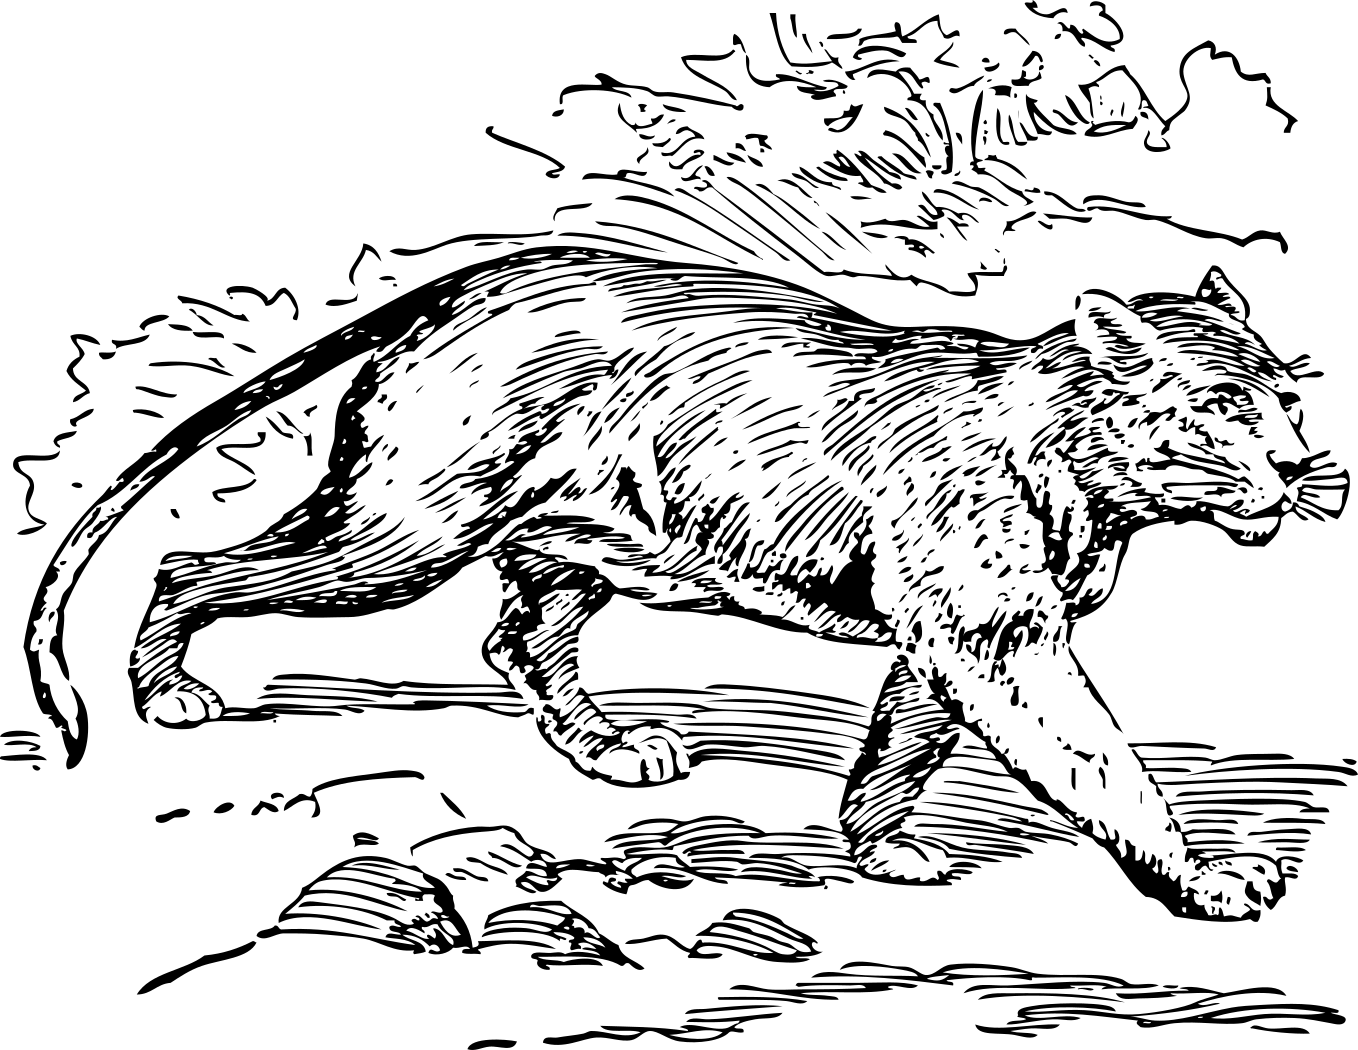
\includegraphics[width = 1\textwidth, left]{../pictures/cheetah.png}
            \end{subfigure}
            \begin{subfigure}{0.5\textwidth}
                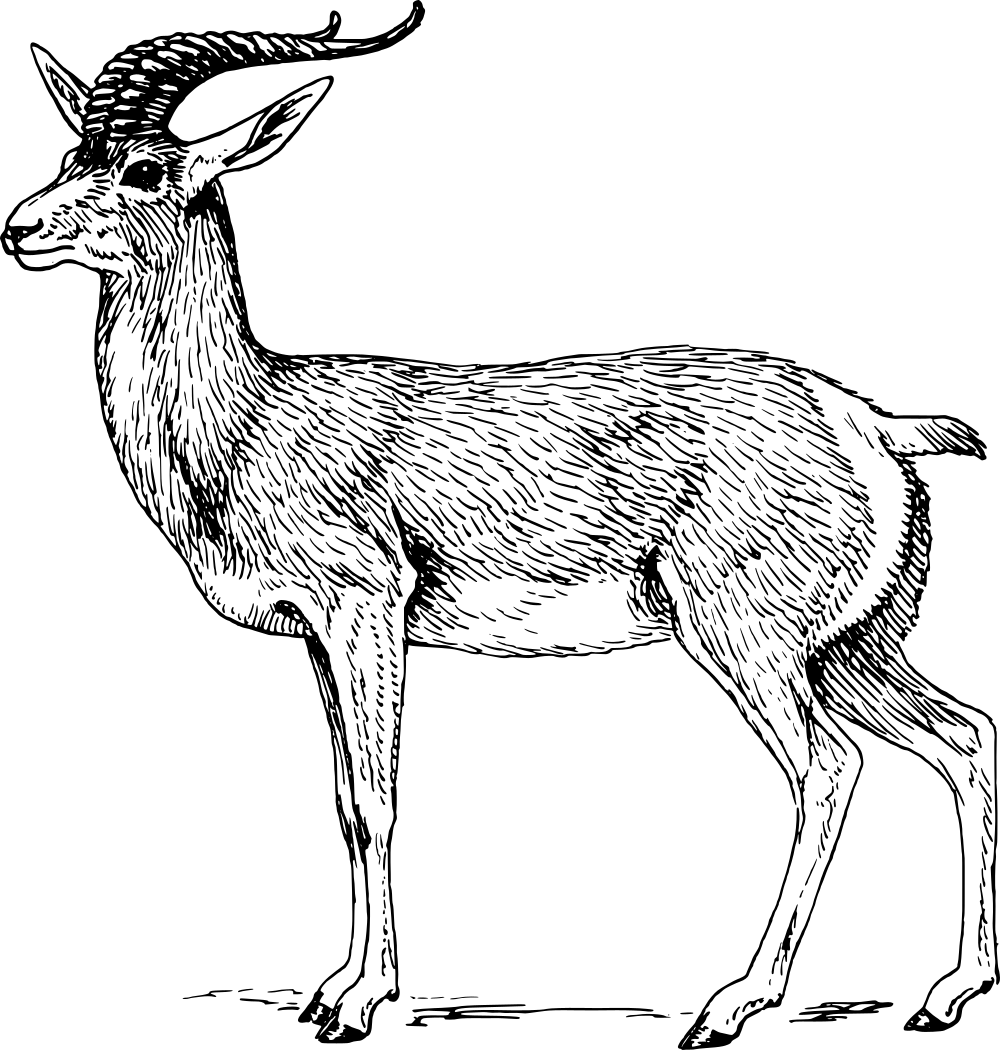
\includegraphics[width = 0.73\textwidth, right]{../pictures/gazelle.png}
            \end{subfigure}
            \caption{Illustration eines Geparden und einer Gazelle \label{fig:gazelleAndGepard}}
        \end{figure}
        \noindent
        Sei unser Gepard durch seine Geschwindigkeit den Gazellen überlegen, dann wird die Gazellenherde über Zeit in ihrer Anzahl sinken. Dabei werden die langsamen Gazellen dem Geparden erliegen und die Schnelleren überleben. Dieser Schritt wird als \textbf{Selektion} bezeichnet. Die Überlebenden werden sich fortpflanzen und mit hoher Wahrscheinlichkeit Gazellen-Babies bekommen die ähnlich schnell sind. Diesen Vorgang bezeichnen wir als \textbf{Kreuzung}. Mit welcher Wahrscheinlichkeit jedes einzelne Tier vor dem Geparden entwischen kann nennen wir \textbf{Fitness}.\\
        \\
        Jede Gazelle, oder auch \textbf{Individuum} genannt, hat eine eigene Fitness, die es aber bei Geburt noch nicht weiß, da sie noch nie vor einem Geparden weglaufen musste. Erst nachdem sie einmal erfolgreich entwischt ist, können wir uns vorstellen, was ihre Fitness ist.\\
        \\
        Ganz selten wird ein Gazellen-Baby geboren, das ein etwas längere Beine hat als alle anderen, dabei hatte keiner dieses Merkmal vor ihr. Das erlaubt ihr schneller zu laufen, was für sie erstmal positiv ist. Diese Ausprägung hat jedoch den Nachteil, dass die Standhaftigkeit darunter leidet. Diese unerwartete Veränderung bei den Kindern heißt \textbf{Mutation}.\\
        \\
        Fassen wir zusammen: Nachdem jede überlebte Gazelle sich fortgepflanzt hat, bekommen wir hoffentlich wieder eine vollzähliges Herde, die wir \textbf{Population} nennen. Nach all diesen Schritten fängt der Kampf um das Überleben wieder an und geht solange, bis sich entweder Gazellen entwickeln, die dem Gepard ständig entkommen können, oder bis die gesamte Population ausstirbt.\\
        \\
        Damit haben wir die wichtigsten Begrifflichkeiten von einem genetischen Algorithmus erklärt und kommen zur Umsetzung der einzelnen Schritte.

        \subsection{Individuen}

            Ein Individuum besteht aus einer Kodierung, auch \textbf{Zustandsraum} genannt, die die aussagekräftigen Eigenschaften von ihm ausmachen. Für eine Gazelle wäre beispielweise die folgende Kodierung möglich.

            \begin{multicols}{2}
                \hfill \\[-10mm]
                \begin{table}[H]
                    \begin{center}
                    \begin{tabular}{ |l|r| } 
                        \hline
                        Höchstgeschwindigkeit    & $ 95\; \frac{km}{h}$   \\ \hline
                        Beinlänge                & $ 86\; cm          $   \\ \hline
                        Gewicht                  & $ 43\; kg          $   \\ \hline
                        Hornlänge                & $ 12\; cm          $   \\ \hline
                    \end{tabular}
                    \end{center}
                    \caption{Kodierung einer Gazelle \label{fig:gaz-encoding}}
                \end{table}

                \noindent
                Die Aufgabe von unserem GA ist ein oder mehrere Individuen zu finden, die es schaffen vor dem Geparden wegzulaufen. Da wir aber nicht wissen, ob die vorgeschlagene Kodierung gut oder schlecht ist, müssen wir Gazellen mit zufälligen Eigenschaften erstellen und dann den Algorithmus arbeiten lassen.
            \end{multicols}
            \noindent
            Das schaffen wir, indem wir Grenzen für die Kodierung festlegen und später zufällige Werte in diesen Rahmen ausprobieren.

            \begin{table}[H]
                \begin{center}
                \begin{tabular}{ |l|r|r| } 
                    \hline
                    Eigenschaft              & Minimaler Wert        & Maximaler Wert       \\ \hline
                    Höchstgeschwindigkeit    & $ 20\; \frac{km}{h}$  & $ 100\; \frac{km}{h}$ \\ \hline
                    Beinlänge                & $ 40\; cm          $  & $ 90\; cm          $ \\ \hline
                    Gewicht                  & $ 12\; kg          $  & $ 75\; kg          $ \\ \hline
                    Hornlänge                & $  0\; cm          $  & $ 35\; cm          $ \\ \hline
                \end{tabular}
                \end{center}
                \caption{Grenzen für die Kodierung \cite{wiki:gazelle} \cite{blog:gazelle}\label{fig:gazelle-bounds}}
            \end{table}
            \noindent
            % Für die Kodierung unseres Individuums eignet sich ein Array von Zahlen. Um die gesamte Population darzustellen würde ein 2-dimensionales Array reichen, wobei jedes Element ein einzelnes Individuum darstellt. \textit{(evtl Grafik)}

        \subsection{Evaluation}
            Nachdem wir unsere Gazellenpopulation erstellt haben, müssen wir sie der Natur überlassen. Dann ist es unsere Aufgabe nach einer festen Zeitspanne und sie alle wieder aufzusammeln. Dadurch finden wir heraus wie viele Gazellen überlebet haben und können diese Information den nächsten genetischen Methoden übergeben.

        \subsection{Selektion}

            Nachdem die Evaluation vorbei ist, bekommen wir die Rückmeldung welche Gazellen überlebt haben. Aus dieser Menge können wir nun einen prozentualen Betrag wählen, die Eltern sein werden. In unserer Implementierung nennen wir diesen Parameter $\alpha$. Damit versichern wir, dass nur die erfolgreichen Eigenschaften weiter in der Population erhalten bleiben und der Rest wegfällt.

        \subsection{Kreuzung}
            Die erfolgreichen Individuen wurden ausgewählt und können sich nun fortpflanzen. Dafür nehmen wir jeweils zwei Individuen und vertauschen zufällig ihre Ausprägungen.
            \\[8mm]
            \begin{multicols}{2}
                \begin{table}[H]
                    \begin{center}
                    \begin{tabular}{ |r| } 
                        \hline
                        \hfill Eigenschaften  \\ \hline
                        \cellcolor{blue!25} $ 56\; \frac{km}{h}$ \\ \hline
                        \cellcolor{blue!25} $ 42\; cm          $ \\ \hline
                        \cellcolor{blue!25} $ 51\; kg          $ \\ \hline
                        \cellcolor{blue!25} $ 10\; cm          $ \\ \hline
                    \end{tabular}
                    \end{center}
                    \caption{Kodierung des Vaters \label{fig:enc-dad}}
                \end{table}

                \begin{table}[H]
                    \begin{center}
                    \begin{tabular}{ |r| } 
                        \hline
                        \hfill Eigenschaften  \\ \hline
                        \cellcolor{yellow!25} $ 62\; \frac{km}{h}$ \\ \hline
                        \cellcolor{yellow!25} $ 55\; cm          $ \\ \hline
                        \cellcolor{yellow!25} $ 49\; kg          $ \\ \hline
                        \cellcolor{yellow!25} $  8\; cm          $ \\ \hline
                    \end{tabular}
                    \end{center}
                    \caption{Kodierung der Mutter \label{fig:enc-mom}}
                \end{table}

            \end{multicols}

            \begin{multicols}{2}
                \begin{table}[H]
                    \begin{center}
                    \begin{tabular}{ |r| } 
                        \hline
                        \hfill Eigenschaften  \\ \hline
                        \cellcolor{blue!25}   $ 56\; \frac{km}{h}$ \\ \hline
                        \cellcolor{yellow!25} $ 55\; cm          $ \\ \hline
                        \cellcolor{yellow!25} $ 49\; kg          $ \\ \hline
                        \cellcolor{blue!25}   $ 10\; cm          $ \\ \hline
                    \end{tabular}
                    \end{center}
                    \caption{Kodierung vom Kind Nr.1 \label{fig:child-1}}
                \end{table}


                \begin{table}[H]
                    \begin{center}
                    \begin{tabular}{ |r| } 
                        \hline
                        \hfill Eigenschaften  \\ \hline
                        \cellcolor{yellow!25} $ 62\; \frac{km}{h}$ \\ \hline
                        \cellcolor{blue!25}   $ 42\; cm          $ \\ \hline
                        \cellcolor{blue!25}   $ 51\; kg          $ \\ \hline
                        \cellcolor{yellow!25} $  8\; cm          $ \\ \hline
                    \end{tabular}
                    \end{center}
                    \caption{Kodierung vom Kind Nr.2 \label{fig:child-2}}
                \end{table}
            \end{multicols}
            \noindent
            Das können wir nun sooft machen wie wir Eltern finden, oder bis wir genug Kinder produziert haben.

            \newpage
            In unserem Beispiel haben wir die Kinder mit dem folgenden Python-Code konstruiert:
            \hfill \\
            \begin{mdframed}
            \begin{minted}[escapeinside=||, linenos]{python}
vater  = [56,42,51,10]
mutter = [62,55,49,8]
kind1  = []
kind2  = []
for i in range(kodierung.length):
    r = random.uniform(0,1)
    if (r > 0.5):
        kind1[i] = vater[i]
        kind2[i] = mutter[i]
    else:
        kind1[i] = mutter[i]
        kind2[i] = vater[i]
            \end{minted}
            \end{mdframed}
            \hfill \\[4mm]
            \noindent
            In \textit{Z.1-2} definieren wir die Eigenschaften der Mutter und des Vaters. Dann iterieren wir durch die Länge der Kodierung (\textit{Z.5}) und wählen mit einer 50\% Wahrscheinlichkeit (\textit{Z.6-7}) aus für jedes Kind aus, ob die gewählte Eigenschaft vom Vater oder von der Mutter kommt.\\

            \noindent
            Diese Art und Weise zwei Individuen zu kreuzen nennt sich \textbf{n-point crossover}, weil wir die Kodierung an zufällig vielen Stellen unterbrechen. Es gibt noch andere Kreuzungsmethoden die eine eine feste Anzahl von Aufteilungen benutzen, wie \textbf{one-} oder \textbf{two-point crossover}. \\
            \\
            \noindent
            Um einen Unterschied zwischen diesen Methoden zu erkennen, stellen wir uns vor dass die Beinlänge im Zusammenhang mit der Höchstgeschwindigkeit steht, weil längere Beine eine größere Sprungweite ermöglichen. Wenn nun ein Kind gezeugt wird, dass lange Beine vererbt, wird die Höchstgeschwindigkeit dadurch nicht automatisch angepasst. Deshalb wäre es besser, wenn diese Ausprägungen zusammen übernommen werden, weil dadurch eine höhere Fitness garantiert werden kann. Kreuzungsmethoden wie n-point-crossover verletzen diese Eigenschaft eher als wie one-point-crossover.\\
            \\
            \noindent
            Je nach Implementierung verwendet man nur eins der beiden Kinder, weil das die Varianz der Gesamtpopulation weniger beeinflusst und trotzdem keinerlei Information verloren geht, weil die Eltern die Kodierung weiter tragen.

\newpage
        \subsection{Mutation}
%            ``Mutation ist hilfreich um die Varianz der Population etwas zu erhöhen'' \\
            Nachdem die Kinder erstellt wurden, müssen wir die Kodierung der Individuen etwas verändern, damit die Varianz in der Gesamtpopulation erhöht wird. Das machen wir indem wir durch die Kodierung der Kinder durchgehen und jede Ausprägung mit einer geringen Wahrscheinlichkeit verändern. Diese nennen wir $\beta$.

            \hspace*{-2cm}
            \begin{multicols}{2}
                \begin{table}[H]
                    \begin{center}
                    \begin{tabular}{ |r| } 
                        \hline
                        \hfill Eigenschaften  \\ \hline
                        \cellcolor{yellow!25} $ 62\; \frac{km}{h}$ \\ \hline
                        \cellcolor{blue!25}   $ 42\; cm          $ \\ \hline
                        \cellcolor{blue!25}   $ 51\; kg          $ \\ \hline
                        \cellcolor{yellow!25} $  8\; cm          $ \\ \hline
                    \end{tabular}
                    \end{center}
                    \caption{Kodierung von einem Kind \label{fig:child-enc}}
                \end{table}

                \begin{table}[H]
                    \begin{center}
                    \begin{tabular}{ |r| } 
                        \hline
                        \hfill Eigenschaften  \\ \hline
                        \cellcolor{yellow!25} $ 62\; \frac{km}{h}$ \\ \hline
                        \cellcolor{blue!25}   $ 42\; cm          $ \\ \hline
                        \cellcolor{red!25}    $ 45\; kg          $ \\ \hline
                        \cellcolor{yellow!25} $  8\; cm          $ \\ \hline
                    \end{tabular}
                    \end{center}
                    \caption{Mutierte Kodierung vom Kind\label{fig:mut-child-enc}}
                \end{table}
            \end{multicols}

            Die Mutation kann folgendermaßen in Python umgesetzt werden:
            \begin{mdframed}
            \begin{minted}[escapeinside=||, linenos]{python}
kinder = [k1, k2...]
beta   = 0.1
for i in range(kinder.length):
    for j in range(kodierung.length):
        r = random.uniform(0,1)
        if (r > beta):
            kinder[i][j] = sampleNewFrom(kodierung[j].range)
            \end{minted}
            \end{mdframed}
            \hfill \\[1mm]
            \noindent
            In \textit{Z.1-2} definieren wir Mutationswahrscheinlichkeit und die Kinder. Dann gehen wir jede Kodierung von jedem Kind durch (\textit{Z.3-4}) und verändern die Eigenschaft mit einer 10\% Wahrscheinlichkeit (\textit{Z.5-7}).\\

            \noindent
            Dieser Schritt ist wichtig, sodass trotz konvergierter Population neue Eigenschaften ausprobiert werden, da sie vielleicht eine bessere Lösung bieten. Der GA tendiert oft dazu sich erstmal für eine suboptimalen Lösung zu entscheiden und die Mutation erlaubt uns einen Ausweg daraus. \\

            \noindent
            In manchen Fällen kann man die Mutation noch weiter parametrisieren, indem man ein Veränderungsfaktor als Argument hinzufügt. Diese Technik benutzt man, wenn die Kodierung nicht trivialerweise verändert werden kann, da sonst bestimmte Eigenschaften verloren gehen. In Kapitel 3 wird genau so ein Fall besprochen, weil wir unsere Individuen durch eine Wahrscheinlichkeitsverteilung darstellen. 

\newpage

        \subsection{Repopulation}
            Die Eltern wurden ausgewählt, die Kindern gezeugt und mutiert, nun müssen wir die Population in eine Form bringen, sodass die Evaluation neu gestartet werden kann. Wir stellen das Problem wieder an einem Beispiel dar.\\

            \begin{mdframed}
            \begin{minted}[escapeinside=||, linenos]{python}

population = [i1,i2,...]                  # population.length = 10
alpha      = 0.4
eltern     = selection(population, alpha) # eltern.length = 4
kinder     = crossover(eltern)            # kinder.length = 4
beta       = 0.1
mutkinder  = mutation(kinder, beta)       # mutkinder.length = 4

newpopulation = eltern + mutkinder        # newpopulation.length = 8
            \end{minted}
            \end{mdframed}
            \hfill \\
            \noindent
            Wir sehen dass uns zwei Individuen weniger als zu Anfang haben können deshalb die Evaluation nicht neu starten. Dieses Problem kann man auf viele Weisen angehen, die ihre eigenen Vorteile und Nachteile haben. 

            \subsubsection*{Mehr Kinder erstellen}
                Es ist möglich während der Kreuzung solange Kinder zu erzeugen, bis die Population wieder ihre Ausgangsgröße angenommen hat. Ein Vorteil wäre, dass diese Individuen mit wahrscheinlich besseren Ausgangskodierungen starten als Neue. Der Nachteil ist jedoch die gesenkte Varianz in der Population und die erhöhte Wahrscheinlichkeit zum Feststecken in einem suboptimalen Lösungen.

            \subsubsection*{Nicht selektiere Individuen nachfüllen}
                Man kann die nicht benutzen Individuen aus der vorherigen Population zum Auffüllen benutzen, was sich aber nur dann gewählt werden sollte, wenn die Chance bestünde, dass sie in der erneuten Simulation besser abschneiden als bisher. Ansonsten nehmen sie den Platz für ein potenziell besseres Individuum weg.

            \subsubsection*{Neue Individuen erstellen}
                In unserer Implementierung haben wir uns für das Nachfüllen von völlig neuen Individuen entschieden, da dadurch die Varianz der Population angehoben wird und dadurch mehr Lösungen möglich sind. Ein Nachteil ist dabei sind die potenziellen Kinder die  keinen Platz bekommen, aber da dadurch keine Information verloren geht, können wir es vernachlässigen.
\newpage

    \section{Neuroevolution}
%        ``Neuroevolution beschäftigt sich mit der Verknüpfung von Genetischen Algorithmen und Neuronalen Netzn''
        Der Begriff der Neuroevolution wurde im Jahre 1988 von D. Whiteley \cite{whiteley88} als alternative Möglichkeit zum Trainieren von künstlichen neuronalen Netzen (\textbf{KNNs}) vorgeschlagen. Dabei wird versucht aus der Synergie von dem \textbf{selbstlernenden Charakter} von KNNs und der \textbf{explorativen Suche} eines GAs eine Taktik oder ein Klassifikator zu entwickeln der völlig neue Lösungen finden kann. Den Beweis dafür hat man bereits im Jahr 1995 am Spiel \textit{Othello} festgestellt. \cite{othello95} \\[2mm]
        \noindent
        Wir versuchen in diesem Kapitel einen groben Überblick über die Funktionsweise von KNNs zu verschaffen und stellen den Bezug zu genetischen Algorithmen dar. Eine weitaus formalere Erklärung findet sich im Paper von ....

        \subsection{Künstliche neuronale Netze}

            Die Idee hinter künstlichen neuronalen Netzen ist der Versuch die Struktur vom menschliche Gehirn nachzuahmen. Ein übliches KNN besteht jedoch aus vielfach weniger Neuronen, meist hundert bis mehrere tausend, wobei unser Gehirn 86 Milliarden\cite{brainsize} besitzt.\\
            \noindent
            Ein künstliches Neuron kann man sich anschaulich als eine Formel vorstellen, die \textbf{eine oder mehrere Eingaben} über \textbf{gewichtete Pfade} bekommt, sie \textbf{aufsummiert} und eine Aktivierungsfunktion auf das Ergebnis anwendet, die auf den Bereich $[0,\infty]$, $[0,1]$, oder $[-1,1]$ abbildet. Dieses Resultat nennen wir $\hat{y}$:

            \begin{figure}[H]
                \begin{mdframed}
                    \noindent
                    Sei $n$ die Anzahl der Eingaben,\\
                    \hspace*{4.5mm}    $X = \{x_0,x_1,...,x_n\}$ die Eingabe,\\
                    \hspace*{4.5mm}    $W = \{w_0, w_1,...,w_n\}$ die jeweiligen Gewichte, \\
                    \hspace*{4.5mm}    $\sigma(x) = max(x,0)$ als Aktivierungsfunktion:\\[4mm]
                    \hspace*{50mm} \Resize{4.5cm}{$\widehat{y} = \sigma(\sum^{n}_{i = 0} x_i \cdot w_i)$}
                \end{mdframed}
                \caption{\label{neuron-math} Formel zur Berechnung des Ergebnisses eines Neurons}
            \end{figure}

            \noindent
            Wenn man nun mehrere von diesen Neuronen in Reihe zusammenschaltet (Abbildung \ref{fig:nntikz}), kriegt man ein vollständig vermaschtes Netz, welches grundsätzlich in drei Schichten unterteilt werden kann.
            \begin{itemize}
                \setlength{\itemsep}{5pt}
                \item \textbf{Eingabeschicht} \\
                    Hier kommt der Ausgangszustand rein, sei es ein kodierter Zustand eines Spiels, RGB Werte von einem Bild, oder der DAX.
                \item \textbf{Versteckte Schicht(en)} \\
                    Dieser Teil des Netzes besteht oft aus mehreren Schichten, da er für die Abstraktion und die Lernfähigkeit verantwortlich ist \cite{ANNModeling}. Er bekommt die Signale aus der Eingabeschicht, die er verarbeitet und weiterleitet. Je nachdem, welche Neuronen dabei \textit{feuern}, beeinflusst das Endergebnis stark.
                \item \textbf{Ausgabeschicht} \\
                    Die Ausgabeschicht ist oft zum Sammeln der Signale von der vorherigen Schicht zuständig und auf ihren Ergebnissen wird dann eine \textbf{Aktivierungsfunktion} angewendet, die die kumulierten Resultate in eine passende Form bringt. Sie varrieren zwischen einfachen Ja/Nein Aussgagen, oder wie wir später kennen lernen werden, auch Wahrscheinlichkeitsverteilungen.

            \end{itemize}

            \tikzset{%
              input neuron/.style={
                circle,
                draw,
                minimum size=1cm,
                fill=inputnode
              },
              hidden neuron/.style={
                circle,
                draw,
                minimum size=1cm,
                fill=hiddennode
              },
              output neuron/.style={
                circle,
                draw,
                minimum size=1cm,
                fill=outputnode
              },
              neuron missing/.style={
                draw=none, 
                scale=1.97,
                text height=0.333cm,
                execute at begin node=\color{black}$\vdots$,
                fill=missingnode
              },
              perceptron/.style={
                circle,
                draw,
                scale=3,
                minimum size=1cm,
                fill=perceptronnode
              }
            }

            \begin{figure}[H]
            \centering
                \begin{tikzpicture}[x=1.5cm, y=1.5cm, >=stealth]
                    \foreach \m/\l [count=\y] in {1,2,3,missing,4}
                        \node [input neuron/.try, neuron \m/.try] (input-\m) at (0,2.5-\y) {};
                    \foreach \m [count=\y] in {1,missing,2}
                        \node [hidden neuron/.try, neuron \m/.try ] (hidden-\m) at (2,2-\y*1.25) {};
                    \foreach \m [count=\y] in {1,missing,2}
                        \node [output neuron/.try, neuron \m/.try ] (output-\m) at (4,1.5-\y) {};
                    \foreach \l [count=\i] in {1,2,3,n}
                        \draw [<-] (input-\i) -- ++(-1,0)
                            node [above, midway] {$x_\l$};
                    \foreach \l [count=\i] in {1,m}
                        \node [above] at (hidden-\i.north) {$h_\l$};
                    \foreach \l [count=\i] in {1,k}
                        \draw [->] (output-\i) -- ++(1,0)
                            node [above, midway] {$y_\l$};
                    \foreach \i [count=\n] in {1,...,4}
                        \foreach \j [count=\m] in {1,...,2}
                            \draw [->] (input-\i) -- node [sloped, above] {$w_{\n,\m}$} (hidden-\j);
%                            \ifthenelse{\n=1}{
%                                \draw [->] (input-\i) -- node [midway, sloped, above=0.3mm] {$w_{\n,\m}$} (hidden-\j);
%                            }{
%                                \draw [->] (input-\i) -- (hidden-\j);
%                            }
                    \foreach \i [count=\n] in {1,...,2}
                        \foreach \j [count=\m] in {1,...,2}
                            \draw [line width = 0.0mm, ->] (hidden-\i) -- node [midway, sloped, above=0.3mm] {$v_{\n, \m}$} (output-\j);
                    \foreach \l [count=\x from 0] in {Eingabe, Versteckte, Ausgabe}
                        \node [align=center, above] at (\x*2,2) {\l \\ Ebene};
                \end{tikzpicture}
                \caption{Skizze von einem vollständig vermaschten künstlichen neuronales Netz \label{fig:nntikz}}
            \end{figure}
            \noindent
            Neuronen wie in Abbildung \ref{fig:nntikz} zusammen zu verknüpfen nennt sich ein \textbf{Feedforward} Netzwerk, da es keine Zyklen beinhaltet. Sie besitzen die Einschränkung das sie ohne Rücksicht auf die resultierenden Effekte in der Domäne ein Ergebnis liefern, da sie das Signal nur nach vorne weiterleiten.\\

            \noindent
            Um eigene Resultate und zeitliche Abstraktionen einfacher zu berücksichtigen gibt es \textbf{rekurrente Netze} die direkte Zyklen beinhalten.

            \subsubsection*{LSTM Ebene}
                Ein spezielles Neuron aus dem rekurrente Netze bestehen können, ist das \textbf{Long Short Term Memory} (LSTM) Neuron\cite{lstm}. Es zeichnet sich durch die Eigenschaft aus, dass es über lange Zeitfenster Information behalten kann. Der Aufbau basiert auf dem Modell einer Speicherzelle, sodass wir durch verschiedene Eingänge (\textbf{Gates}), die Schreib-,Lese- und Reset-Aktionen nachbauen können \cite{lstm-new}. Einer der wichtigste Aspekte von diesen Neuronen ist jedoch, dass sie ableitbar sind, weil dadurch die Trainingsmethode \textbf{Backpropagation} ermöglicht wird \cite{backprop}.

\newpage
            \subsubsection*{Backpropagation}
                Um diese Technik zum Trainieren von KNNs zu erklären müssen wir zunächst zeigen wie man den Fehler von einem neuronalen Netz misst. Dafür brauchen wir eine \textbf{Kostenfunktion} die uns die Abweichung zum Soll-Ergebnis gibt. Die Ergebnisse des Netzes für $\widehat{y}$ ist in Abbildung \ref{neuron-math} definiert.

                \begin{figure}[H]
                    \begin{mdframed}
                        \noindent
                        Sei $m$ die Größe des Trainingssets,\\
                        \hspace*{4.5mm} $Y = \{y_0, y_1,...,y_m\}$ ein Vektor von Soll-Ergebnissen, \\
                        \hspace*{4.5mm} $\widehat{Y} = \{\widehat{y}_0, \widehat{y}_1,...,\widehat{y}_m\}$ ein Vektor von Resultaten des KNNs, dann ist:\\[4mm]
                        \hspace*{30mm} \Resize{7cm}{cost$(Y, \widehat{Y}) = \frac{1}{m} \cdot \sum_{j = 0}^{m} \; (y_j - \widehat{y}_j)^2$}\\[4mm]
                        die mittlere quadratische Abweichung.
                    \end{mdframed}
                    \caption{\label{cost-math} Formel zur Berechnung des \textit{MSE} Fehlers von einem KNN}
                \end{figure}
                \noindent
                Eine der möglichen Kostenfunktionen sieht man in Abbildung \ref{cost-math}, die \textbf{mittlere quadratische Abweichung} (MSE). Je kleiner diese Kostenfunktion ist, umso besser kann unser KNN die Ergebnisse nachahmen. Um die Kosten zu minimieren, müssen wir die gesamte Funktion samt der Berechnung vom $\widehat{y}$ partiell nach den Gewichten ableiten. \\[2mm]
                Mit dem resultierenden Gradienten verändern wir die Gewichte, sodass der Fehler möglichst verringert wird. Dafür leiten wir die Anpassungsformel für jedes Gewicht her:

%                 Damit finden wir heraus, wie wir jedes einzelne Gewicht verändern müssen damit am Ende das richtige Ergebnis rauskommt, sodass alles gegen 0 geht. Dafür leiten wir die Anpassungsformel für jedes Gewicht her:

                \begin{figure}[H]
                    \begin{mdframed}
                        \noindent
                        Pro Beobachtung $j$ in $Y$,\\
                        pro Gewicht $i$ in $W$ leiten wir partiell nach $w_i$ ab:\\[4mm]
    \hspace*{40mm} \Resize{5.5cm}{$\frac{\partial \text{cost}(y_j,\widehat{y}_j)}{\partial w_i} = \frac{\partial}{\partial w_i} (y_j - \widehat{y}_j)^2$} \\[2mm]
    \hspace*{62.3mm} \Resize{7.0cm}{$ = \frac{\partial}{\partial w_i} (y_j - max(\sum_{i = 0}^{n} x_i \cdot w_i ,0))^2$} \\[2mm]
    \hspace*{62.3mm} \Resize{6.25cm}{$ = -2 \cdot \frac{\partial}{\partial w_i} \; max(\sum_{i = 0}^{n} x_i \cdot w_i ,0)$} \\[2mm]
    \hspace*{62.3mm} \Resize{6.25cm}{$ =   \begin{cases}
                                            0 & \sum_{i = 0}^{n} x_i \cdot w_i < 0 \\[2mm]
                                            -2 \cdot x_i & \sum_{i = 0}^{n} x_i \cdot w_i > 0 \\
                                        \end{cases}$}\\[4mm]
                        Damit bekommen wir für Anpassungsregel für jedes Gewicht:\\[4mm]
                        \hspace*{40mm} \Resize{6.5cm}{$w_i \leftarrow w_i + \begin{cases}
                                                                               0 & \sum_{i = 0}^{n} x_i \cdot w_i < 0 \\[2mm]
                                                                               -2 \cdot x_i & \sum_{i = 0}^{n} x_i \cdot w_i > 0 \\
                                                                             \end{cases}$}
                    \end{mdframed}
                    \caption{\label{derivative} Berechnung der Anpassungsregel für jedes Gewicht nach MSE}
                \end{figure}


                \noindent
                Diese Technik kann man benutzen, solange das gesamte Netz als Formel dargestellt ableitbar ist, selbst wenn es mehrere versteckte Schichten hat. Leider braucht sie dafür ein Trainingsset von Daten, was in oft aufwendig zu generieren ist. Deshalb benutzen wir eine simulationsbasierte Lernmethode.


            \subsubsection*{Softmax Ebene}
                Es gibt eine Aktivierungsfunktion der wir besondere Aufmerksamkeit widmen, da sie die Neuronen der Ausgabeschicht zu einem nützlichen Ergebnis zusammenfassen kann. Die generalisierte logistische Funktion, oder auch \textbf{normalisierte Exponentialfunktion} nimmt als Argument einen $k$-dimensionalen Vektor \textbf{z} von reelen Zahlen und gibt uns widerrum den gleichen Vektor zurück, wo alle Werte auf den Bereich [0,1] normalisiert wurden.

            \begin{figure}[H]
                \begin{mdframed}
                    Sei $j = 1,2,...,K$: \\
                    \hspace*{45mm} \Resize{4cm}{$\sigma(\textbf{z})_j = \frac{e^{\textbf{z}_j}}{\sum^{K}_{k = 1} e^{\textbf{z}_k}}$}
                \end{mdframed}
                \caption{\label{softmax} Definition der Softmax Funktion}
            \end{figure}

            \noindent
            Aufmerksame Leser fragen sich vielleicht warum man keine einfache Normalisierung vornimmt. Wenn man als Trainingsfunktion bei Backpropagation den logistischen Fehler (\textbf{logistic-loss}) oder \textbf{cross entropy loss} benutzt, kürzt sich das $e$ weg und bietet sich daher an.

        \subsection{Verbindung mit genetischen Algorithmen}
            Wenn wir nun zum Trainieren von ANNs genetische Algorithmen benutzen wollen, müssten wir das Netz als Liste von Gewichten kodieren, aus denen es besteht. Ein Beispiel dafür bietet der \textbf{GENITOR}\cite{moriarty1999evolutionary} Algorithmus. Dabei werden die einzelnen Gewichte der Kreuzung und einer speziellen Mutation ausgesetzt die von der Varianz der Gesamtpopulation abhängt. \\

            \noindent
            Ein weiterer Ansatz ist \textbf{SANE}\cite{moriarty1999evolutionary}, der einzelne Neuronen für die \textit{Hidden Ebene} entwickelt und daraus ein Netz generiert. Dadurch wurde die Mobility-Strategie für das Spiel Othello wiederentdeckt. \\

            \noindent
            Leider benutzen neuronale Netze heutzutage je nach Anwendungsgebiet immer aufwendigere Strukturen die extrem viele Gewichte besitzen. Eine naive genetische Suche in so einem hochdimensionalen Zustandsraum dauert zu lange und deshalb gibt es Techniken die uns erlauben zielsicherer und effizienter den Raum aller Möglichkeiten zu durchsuchen.

%            ``Die Verknüpfung findet in der Kodierung von den Individuen statt - wir nehmen eine (naive) Darstellung von allen Gewichten''
%            ``Problematik -> Folgerung zu DCT''

    \section{Diskrete Kosinus Transformation}
        % ``Der Suchraum kann durch die sog. DCT auf beliebige Dimensionalität eingeschränkt werden, wenn bestimmte Annahmen getroffen werden können'' \\
        % ``Fouriertransformationen machen folgendes...'' \\
        % ``Es gibt eine Inverse die aus einem n-stelligen liste eine m-stellige macht, wo die Zahlen korelliert sind (Beispiele)''

        Eine dieser Techniken ist die Nutzung der diskreten Kosinustransformation (\textbf{DCT}), die zur Familie der Fouriertransformationen gehört. Eine \textbf{Fouriertransformation} spaltet ein Signal in beliebig viele trigonometrische Funktionen, wie Sinus oder Kosinus und über die Summe dieser Funktionen kann jede mögliche Ausprägung von Daten beschrieben werden. \\

        \noindent
        Diese Fouriertransformation liefert uns dadurch ein diskretes Frenquenzenspekturm, das in Form von Koeffizienten dargestellt wird. Dabei wird pro kodierter Datenpunkt ein Koeffizient benutzt. Um die Daten wiederherzustellen gibt es die inverse Kosinustransformation die die Koeffizienten wieder umwandelt.

        \begin{multicols}{2}
            \begin{figure}[H]
                \begin{center}
                    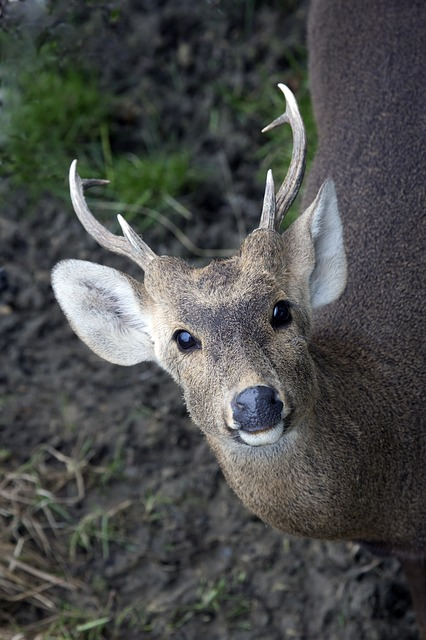
\includegraphics[scale=1]{../pictures/gazelle-uncompressed.jpg}\\
                    \caption{Unkomprimiert}\label{fig:gazelle-uncompressed}
                \end{center}
            \end{figure}
            \par
            \begin{figure}[H]
                \begin{center}
                    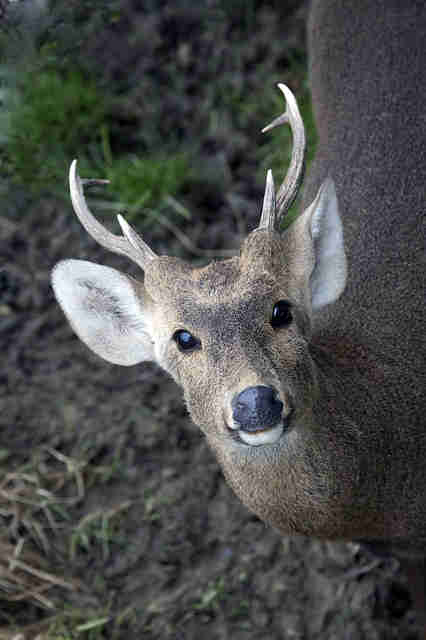
\includegraphics[scale=0.239]{../pictures/gazelle-compressed.jpg}\\
                    \caption{Komprimiert (1:5)}\label{fig:gazelle-compressed}
                \end{center}
            \end{figure}
        \end{multicols}

        \noindent
        Wenn wir viele der Koeffizieten nicht benutzen und trotzdem versuchen die Datenpunkte wiederherzustellen, kriegen wir lediglich eine Annäherung, wie man in Abbildung \ref{fig:gazelle-compressed} sieht. Sie ist meistens aber so gut genug, dass wir keinen Unterschied merken. Eine sehr ähnliche Kompressionsmethode kennt man aus dem Bildformat JPEG oder dem Videoformat MPEG.

        \subsection{Kodierung des Suchraums}

            Diese Technik wenden wir nun auf die Gewichte von unserem neuronalen Netz an. Dafür beschränken wir den Suchraum auf eine kleine Anzahl der Koeffizienten und benutzen die inverse Kosinustransformation um aus ihnen die nötige Anzahl von Gewichten zu erstellen. In Abbildung \ref{fig:dct-pre},\ref{fig:dct-after} sieht man eine Anwendung auf 100 Gewichte die in einem Verhältnis von 1:2 komprimiert wurden. Das bedeutet dass wir den Suchraum mit dem sichtbaren Genauigkeitsverlust halbiert haben.\\

            \noindent
            Bei größeren Verhältnissen bemerken wir eine starke örtliche Korrelation (\ref{fig:dct-my-case}) zwischen den benachbarten Zahlen und diese Eigenschaft passt zu der Annahme dass sich Gewichte in neuronalen Netzen ähnlich verhalten. Eine ausführlichere Erklärung findet sich im Ursprungspaper für die Anwendung in der Neuroevolution.\cite{cosyne1}
            \begin{multicols}{2}
                \begin{figure}[H]
                    \begin{center}
                        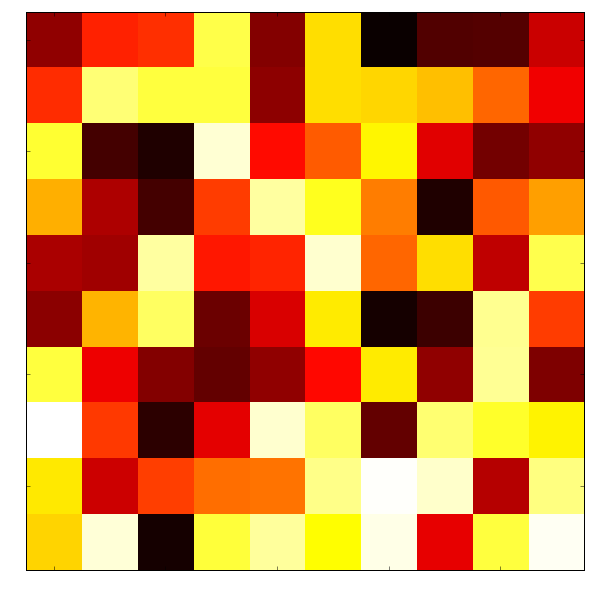
\includegraphics[scale=0.2]{../pictures/DCT-pre.png}\\
                        \caption{Unkomprimiert}\label{fig:dct-pre}
                    \end{center}
                \end{figure}
                \par
                \begin{figure}[H]
                    \begin{center}
                        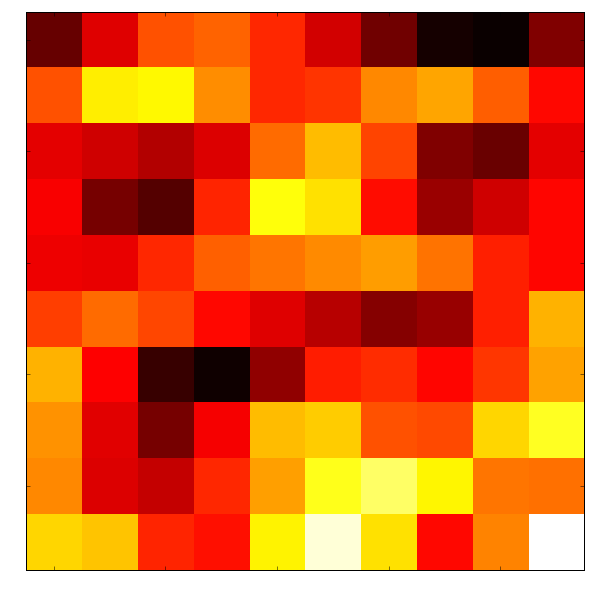
\includegraphics[scale=0.2]{../pictures/DCT-after.png}\\
                        \caption{Komprimiert (1:2)}\label{fig:dct-after}
                    \end{center}
                \end{figure}
            \end{multicols}

    \section{Cooperative Synapsen Neuroevolution}
%         ``CoSyNE wurde vom Prof.Dr.Schmidhuber an der ETH Zürich entwickelt und hat damit sehr viele anderen Algorithmen in den Schatten gestellt''\\
%        ``Methodik, ist wie GA bloß mit einer Aktion mehr die statt spielbare `Policies', nur im Koeffizientraum entwickle'' \\
%        ``Dies erlaubt eine (zitat) Kooperative Entwicklung von Koeffizienten für die nachfolgenden Inv.DCT'' \\
%        ``Kein Crossover, geringe Mutation'' \\
%        ``Beispiele vom Erfolg'' \\
        Nachdem wir den Zustandsraum komprimiert haben, sodass ein genetischer Algorithmus ihn in absehbarer Zeit entwickeln und ein neuronales Netz befüllt werden kann, erschließt sich die Verküpfung zu einem mächtigen Werkzeug das viele interessante Eigenschaften besitzt. Dieser Algorithmus wird \textbf{Cooperative Synapsen Neuroevolution}\cite{cosyne2}, oder auch \textbf{CoSyNE} genannt.\\

        \noindent
        Er zeichnet sich speziell dadurch aus, dass er auf kontinuierlichen Zuständen und Aktionen funktioniert und spärliche Fitnessignale interpretieren kann. Das schafft er indem er rekurrente Netze aufbaut und die genetische Suche mit aggresiver Mutation im Zustandsraum beschleunigt. Ein gutes Beispiel dafür ist das Rennspiel \textbf{TORCS}\cite{cosyne3} wo der Algorithmus 993 Gewichte in 33 Koeffizienten kodiert \textit{(Faktor 1:30)} und lediglich durch die Bilddaten ähnlich gute Ergebnisse liefert wie die per Hand programmierten Agenten die die Physik des Spieles kennen.\\

        \noindent
        Ein großer Nachteil von genetischen Algorithmen ist das sie oft schnell zu lokalen Maxima konvergieren und sehr schlecht aus diesem Tal rauskommen. Um dieses Problem anzugehen, versucht man die Stellschrauben wie Mutationswahrscheinlichkeit oder Kinderanzahl per Hand zu verändern. CoSyNE benutzt dafür eine ganz eigene \textbf{genetische Methode} um die Suche einfacher zu gestalten. Sie nennt sich Permutation und erzeugt innerhalb der gesamten Population Unterteilungen in kleinere Populationen die in einer \textbf{kooperativen und koevolutionären} Beziehung stehen.
%          \begin{figure}[H]
%              \begin{center}
%                  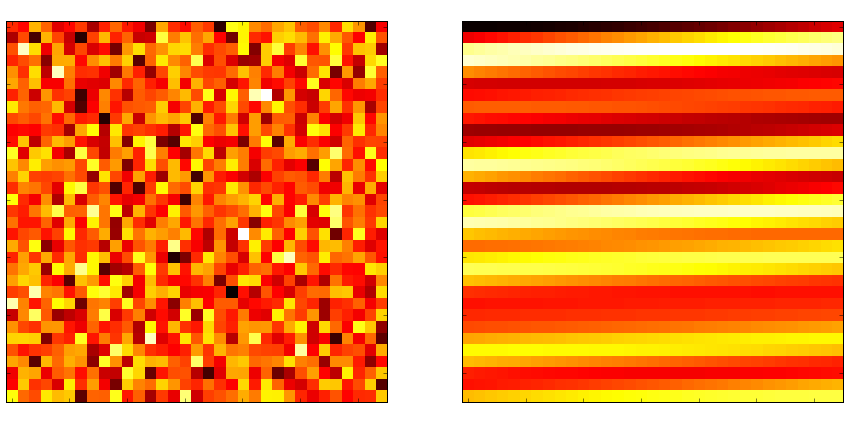
\includegraphics[scale=0.5]{../pictures/DCT-my-case.png}\\
%                  \caption{1024 Gewichte auf 23 Koeffizienten reduziert}\label{fig:dct-my-case}
%              \end{center}
%          \end{figure}
% \newpage
        \subsection{Permutation}
            % ``Wir transponieren, shuffeln und transponieren zurück''
            Der Permutationsschritt wird ganz am Ende von dem genetischen Algorithmus statt der Repopulation aufgerufen und vermischt jeden \colorbox{green!25}{Eigenschaftsraum} der Gesamtpopulation. 

            \begin{table}[H]
                \begin{center}
                \begin{tabular}{ |r|r|r|r|r| } 
                    \hline
                    Individuum & \cellcolor{green!25} Höchstgeschwindigkeit & \cellcolor{green!25} Beinlänge & \cellcolor{green!25} Gewicht & \cellcolor{green!25} Hornlänge \\ \hline
                    $1$        & $60\; \frac{km}{h}$   & $40\; cm$ & $50\; kg$ & $10\; cm$ \\ \hline
                    $2$        & $61\; \frac{km}{h}$   & $41\; cm$ & $51\; kg$ & $11\; cm$ \\ \hline
                    $3$        & $62\; \frac{km}{h}$   & $42\; cm$ & $52\; kg$ & $12\; cm$ \\ \hline
                    $4$        & $63\; \frac{km}{h}$   & $43\; cm$ & $53\; kg$ & $13\; cm$ \\ \hline
                    $5$        & $64\; \frac{km}{h}$   & $44\; cm$ & $54\; kg$ & $14\; cm$ \\ \hline
                    $6$        & $65\; \frac{km}{h}$   & $45\; cm$ & $55\; kg$ & $15\; cm$ \\ \hline
                \end{tabular}
                \end{center}
                \caption{Vor der Permutation \label{fig:pre-perm}}
            \end{table}

            \begin{table}[H]
                \begin{center}
                \begin{tabular}{ |r|r|r|r|r| } 
                    \hline
                    Individuum & \cellcolor{green!25} Höchstgeschwindigkeit & \cellcolor{green!25} Beinlänge & \cellcolor{green!25} Gewicht & \cellcolor{green!25} Hornlänge \\ \hline
                    $1$        & \cellcolor{blue!45} $61\; \frac{km}{h}$   & \cellcolor{yellow!25} $43\; cm$ & \cellcolor{red!15} $54\; kg$ & \cellcolor{violet!45} $12\; cm$ \\ \hline
                    $2$        & \cellcolor{blue!45} $60\; \frac{km}{h}$   & \cellcolor{yellow!45} $44\; cm$ &                    $51\; kg$ & \cellcolor{violet!25} $14\; cm$ \\ \hline
                    $3$        & \cellcolor{blue!15} $64\; \frac{km}{h}$   & \cellcolor{yellow!65} $45\; cm$ & \cellcolor{red!35} $53\; kg$ & \cellcolor{violet!45} $10\; cm$ \\ \hline
                    $4$        &                     $63\; \frac{km}{h}$   & \cellcolor{yellow!25} $40\; cm$ & \cellcolor{red!35} $52\; kg$ & $13\; cm$ \\ \hline
                    $5$        & \cellcolor{blue!15} $62\; \frac{km}{h}$   & \cellcolor{yellow!45} $41\; cm$ &                    $54\; kg$ & \cellcolor{violet!25} $11\; cm$ \\ \hline
                    $6$        &                     $65\; \frac{km}{h}$   & \cellcolor{yellow!65} $42\; cm$ & \cellcolor{red!15} $50\; kg$ & $15\; cm$ \\ \hline
                \end{tabular}
                \end{center}
                \caption{Nach der Permutation \label{fig:pre-perm}}
            \end{table}

            \noindent
            Wenn wir uns die Population als zweidimensionale Liste vorstellen, wo jedes Indviduum eine eigene Liste mit seinen spezifischen Ausprägungen ist, können wir die Population transponieren, wobei nun jede Eigenschaft eine eigene Liste ist, diese vermischen und wieder zurück transponieren um die neuen Individuen zu bekommen. Der folgende Pythoncode veranschaulicht das Prinzip unter Verwendung der \textit{numpy} Bibliothek.

            \begin{mdframed}
            \begin{minted}[escapeinside=||, linenos]{python}
import numpy as np

i_1 = [1,10,100,1000] # Individuum 1-5
i_2 = [2,20,200,2000]
i_3 = [3,30,300,3000]
i_4 = [4,40,400,4000]
i_5 = [5,50,500,5000]

population = np.array([i_1, i_2, i_3, i_4, i_5])
eigenschaftsraum = np.transpose(population)
  
for eig in eigenschaftsraum:
    np.random.shuffle(eig)

population = np.transpose(eigenschaftsraum)

print population
> [[   2   40  500 5000]
   [   1   50  200 1000]
   [   4   10  300 3000]
   [   3   30  100 2000]
   [   5   20  400 4000]]

            \end{minted}
            \end{mdframed}
            \noindent
            Man erkennt leicht, dass keiner der ursprünglichen Individuen erhalten bleibt und wir vollkommen Neue bekommen. Der Sinn hinter dem Verschmischen in der Eigenschaftsebene versteckt sich in der \textbf{Verknüpfungung mit der Kreuzungsmethode}. Wenn wir zwei Individuen kreuzen, werden ihre Kinder sicherlich die gesamte Information von ihren Eltern in der Population übernehmen. Da CoSyNE den Repopulationsschritt nicht ausführt, aber dennoch schlechte Individuen wegwirft, wird irgendwann nur noch die Kodierung von den Kindern übrig bleiben.\\

            \noindent
            Das führt zur Homogenität in den einzelnen Eigenschaften, die zum Beispiel dafür verantworlich ist, dass alle Individuen gleich große Hörner haben. Wenn nun innerhalb der Hornlänge zufällig gemischt wird, bleibt alles gleich, da die gesamte Liste aus dem gleichen Element besteht. \\

            \noindent
            Die Annahme von CoSyNE ist dass die Lösung für das Problem in der Kombination von den Ausprägungen von allen Individuen liegt, die wir am Anfang erstellen. Durch das aggressive Aussortieren durchsuchen wir den Raum aller Möglichkeiten schneller und darin liegt der größte Vorteil von diesem Algorithmus.

\newpage
    \section{Cross Entropy Method}
        Eine andere Möglichkeit die Individuen in dem GA zu kodieren stellt die \textbf{Cross Entropy Method} dar. Das ist ein Algorithmus der oft als Vergleichskriterium verwendet wird, da er oft zu suboptimalen Strategien konvergiert\cite{cem}. Die Anwendung in unserem neuroevolutionären Schema basiert darauf, dass wir Individuen nicht als Ansammlung von Zahlen zu speichern, sondern jede Eigenschaft als Normalverteilung dargestellt wird. Diese Abläufe illustrieren wir anhand der Erklärung für eine Normalverteilung ist.

        \subsection{Normalverteilung}

            Eine Normalverteilung ist eine sehr bekannte stetige Wahrscheinlichkeitsverteilung. Ihre Wahrscheinlichkeitsdichtefunktion wird oft Gauß-Kurve oder Glockenkurve genannt und findet Anwendung in verschiedensten Anwendungsgebieten, weil sie natürliche Vorgänge exakt oder ähnlich genug modelliert. Bekannte Beispiele dafür sind die Streuung von Messfehlern oder die irreguläre Bewegung von Partikeln in einer Flüssigkeit (\textbf{Brownsche Bewegung}).\\

            \noindent
            Die Wahrscheinlichkeitsdichtefunktion der Normalverteilung ist von zwei Parametern abhängig, dem Durchschnitt und der Standardabweichung:

            \begin{figure}[H]
                \begin{mdframed}
                    \noindent
                    Sei $\mu$ der Durchschnitt,\\
                    \hspace*{4.5mm}    $\sigma$ die Standardabweichung, dann ist\\[4mm]
                    \hspace*{50mm} \Resize{6cm}{$\mathcal{N}(x\;|\;\mu, \sigma^2) = \frac{1}{\sqrt{2\pi\sigma^2}} \cdot e^{-\frac{(x - \mu)^2}{2\sigma^2}} $} \\[4mm]
                    \hspace*{4.5mm} die Wahrscheinlichkeitsdichtefunktion der Normalverteilung.
                \end{mdframed}
%                \caption{\label{norm-dist-pdf-formel} Definition der Wahrscheinlichkeitsdichtefunktion der Normalverteilung}
            \end{figure}

            \begin{figure}[H]
                    \begin{center}
                        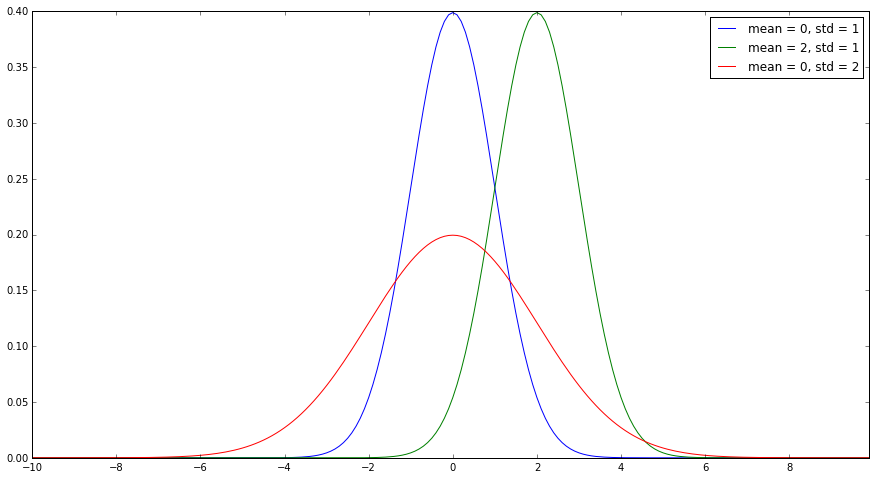
\includegraphics[scale=0.4]{../pictures/diagrams/normal-dist-example.png}\\
                        \caption{Dichtefunktionen von Normalverteilungen}\label{fig:norm-dist-pdf}
                    \end{center}
            \end{figure}

            \noindent
            Die Abbildung (\ref{fig:norm-dist-pdf}) zeigt beispielhafte Ausprägungen der Dichtefunktion, an denen man erkennen kann, dass die Standardabweichung für die Amplitute und der Durchschnitt für die Phase verantwortlich ist. Um die Wahrscheinlichkeit zu berechnen, dass eine zufällige Variable $\mathcal{X}$  mit den Grenzen $a \leq \mathcal{X} \leq b$ eintritt ist:

            \begin{figure}[H]
                \begin{mdframed}
                    \hspace*{40mm} \Resize{6cm}{$P(a \leq \mathcal{X} \leq b) = \int_a^{b} \; \mathcal{N} (\mu, \sigma^2)$}
                \end{mdframed}
                \caption{Wahrscheinlichkeit der Ausprägung $a \leq \mathcal{X} \leq b$}
            \end{figure}

            \noindent
            Diese Formel lässt sich an dem Beispiel von Regenfall pro Quadratmeter veranschaulichen:

            \begin{figure}[H]

                    \begin{center}
                        \hspace{-1cm}
                        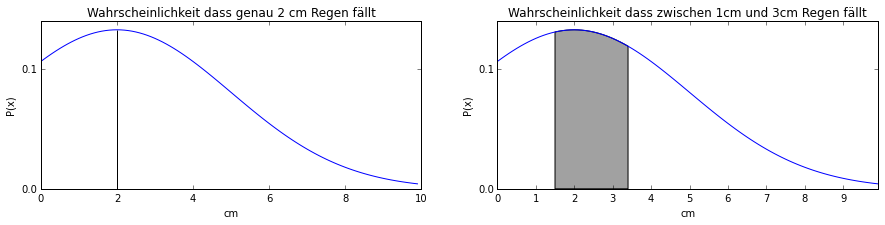
\includegraphics[scale=0.5]{../pictures/diagrams/rainfall-pdf.png}\\
%                        \caption{Kodierung der Eigenschaften durch Normalverteilungen}\label{fig:norm-dist-encoding}
                    \end{center}
            \end{figure}
            \noindent
            Die Wahrscheinlichkeit dass pro Quadratmeter \textit{genau} $2cm$ Regenwasser fällt ist extrem gering, weil nicht ein Yoctometer ($10^{-24})$ mehr oder weniger fallen darf. Wenn wir diese zufällige Ausprägung jedoch als Grenzen definieren, dann steigt die Wahrscheinlichkeit. Die Wahrscheinlichkeit dass zwischen $1cm$ und $3cm$ Regenwasser fällt ist eine viel wertvollere Aussage und ist als Integral zwischen den Grenzen der Dichtefunktion definiert.\\

            \subsubsection*{Kodierung durch Normalverteilungen}

            \begin{figure}[H]
                    \begin{center}
                        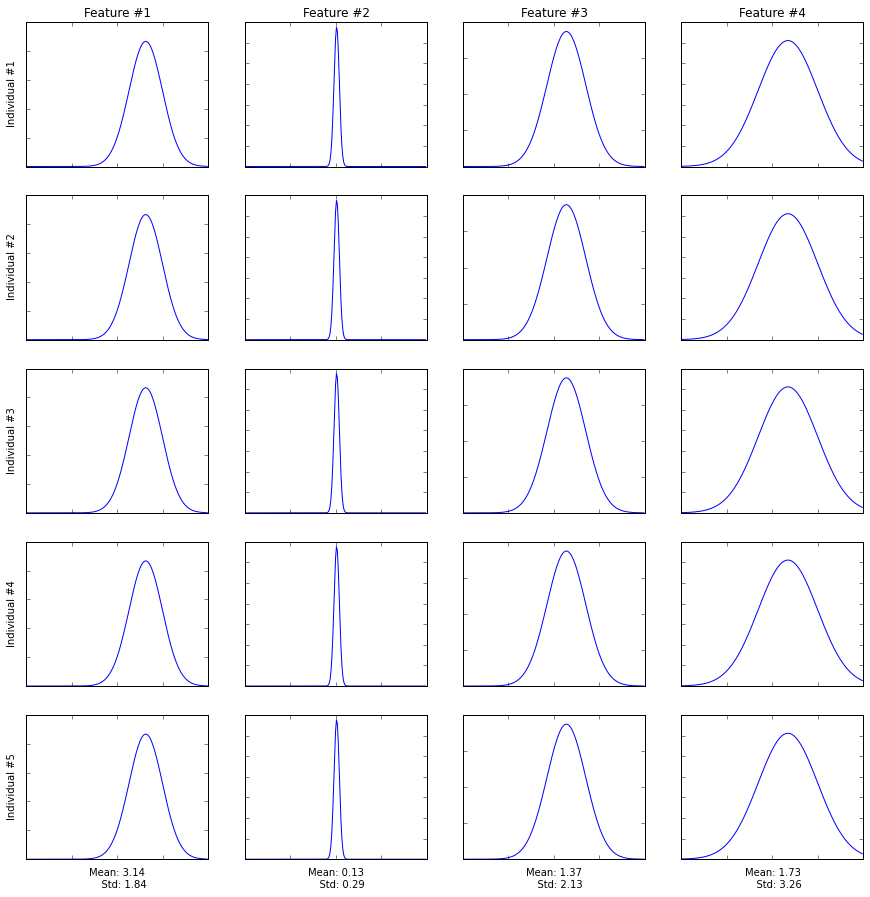
\includegraphics[scale=0.49]{../pictures/diagrams/cross-entropy-visualization-ga.png}\\
                        \caption{Kodierung der Eigenschaften durch Normalverteilungen}\label{fig:norm-dist-encoding}
                    \end{center}
            \end{figure}

            Stellen wir nun die Kodierung der Eigenschaften von jedem Individuum als Normalverteilung dar. Das bedeutet wir haben für jede Eigenschaft, zum Beispiel \textit{Hornlänge}, einen Durchschnitt und eine Standartabweichung. Die Abbilung (\ref{fig:norm-dist-encoding}) zeigt dies beispielhaft für fünf Individuen mit jeweils 4 Eigenschaften dar.\\[3mm]
            \noindent
            Wenn wir Individuen erstellen wollen, müssen wir aus jeder Normalverteilung eine Stichprobe nehmen. Die Kreuzung und Mutation fällt aus, dafür aktualisieren wir nach jeder Simulation alle Verteilungen aus den Durchschnitten und Standartabweichungen der besten Individuen.

    \chapter{Umsetzung in RoboCup2D}
    % ``Was ist RoboCup'' \\
    % ``Was für Ligen gibt es'' \\
    % ``Was für eine Domäne ist es im Vergleich zu anderen'' \\
    % \\
    RoboCup ist ein Fußball Simulator, der seine Anfänge in 1993 in Japan, Tokyo gefunden hat. Eine Gruppe von Forschern, inklusive Minoru Asada, Yasuo Kuniyoshi und Hiroaki Kitano, haben als einen Wettbewerb unter dem Namen \textbf{Robot J-League} gestartet. Der Name stammt von einer professionellen japanischen Fußball Liga.\\
    \\
    Nach einem Monat haben sie jedoch weltweit überwältigendes Feedback bekommen und haben die Initiative als internationales Projekt weitergeführt, daher kam die Umbenennung zur \textbf{Robot World Cup Initiative}, kurz RoboCup. \\
    % \textit {(source: http://www.robocup.org/about-robocup/a-brief-history-of-robocup/)} \\
    \\
    Die RoboCup Initiative hat betreibt derzeit sechs große Wettbewerbe, die sich jeweils wieder in Ligen und Subligen aufteilen lassen. Darunter fällt \textbf{RoboCup Soccer}, \textbf{RoboCup Rescue Rescue}, \textbf{RoboCup Junior}, \textbf{RoboCup Logistics}, \textbf{RoboCup @ Work} und \textbf{RoboCup @ Home}. Unsere Implementierung fällt in die Subliga \textbf{2D Soccer Simulation}, in der es darum geht in einer zweidimensionalen Welt zwei Fußballmannschaften gegeneinander antreten zu lassen.\\
    \\
    Die Aufgabe die wir angehen gehört zu einem Fragement von RoboCup2D, genannt \textbf{Half Field Offense}.\\

    \begin{figure}[htbp]
        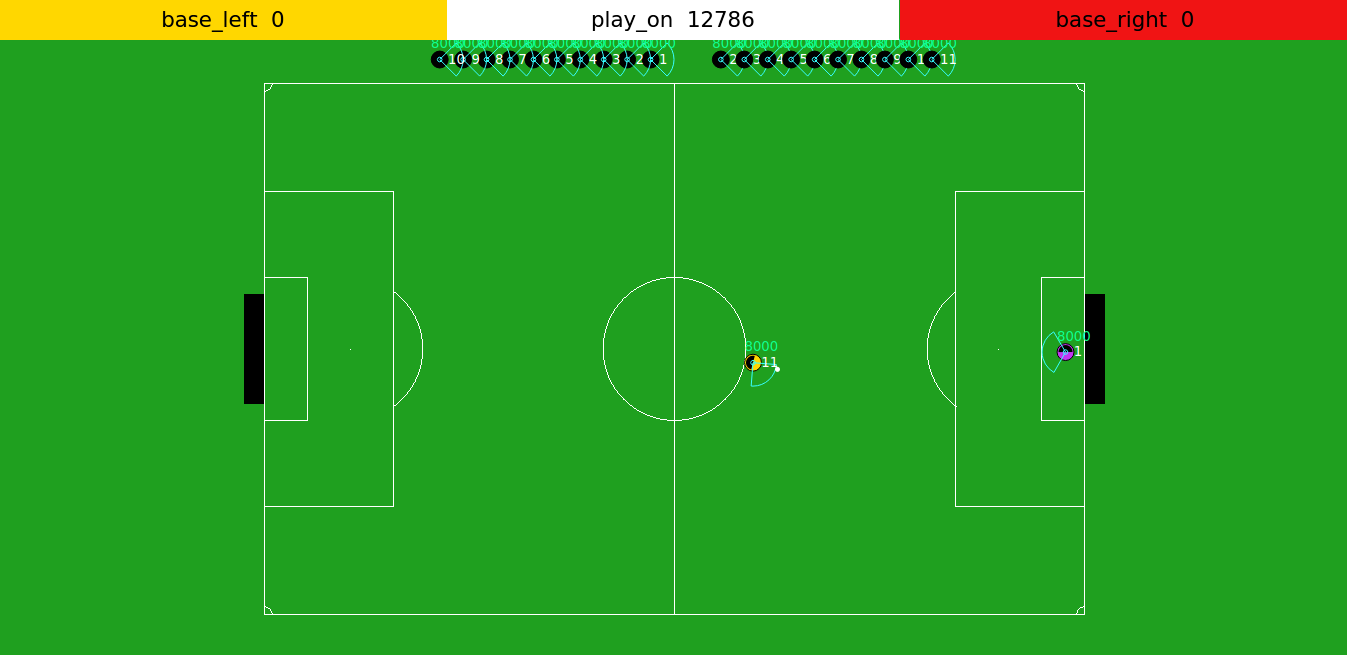
\includegraphics[width = 1.0\textwidth, center]{../pictures/full-field.png}
        \caption{Screenshot von dem gesamten Spielfeld von RoboCup2D \label{fig:somelabel}}
    \end{figure}

    \section{Half Field Offense}
        % ``Was ist Half Field Offense'' \\
        % ``Wie ist das Spielfeld aufgebaut'' \\
        % ``Warum wurde diese Domäne gewählt'' \\

        Die Domäne Half Field Offense grenzt das Spielfeld auf eine Hälfte ein, sodass wir 4 Angreifer und 3 Verteidiger + Torwart haben. Diese Einschränkung vereinfacht den Such- und Zustandsraum immens und erlaubt potenziell eine Wiederverwendbarkeit der Agenten, wenn eine vollständige Mannschaft aufgebaut wird.\\
        \\
        In unserer Implementierung haben wir lediglich ein 1v1 Szenario, also ein Angreifer gegen ein Torwart. Diese sieht jedoch explizit ein nahtlosen Skalierung auf ein 4vs4 Szenario vor, sodass weitere Parametrisierung ohne viel Aufwand ausprobiert werden können.\\

        \begin{figure}[htbp]
            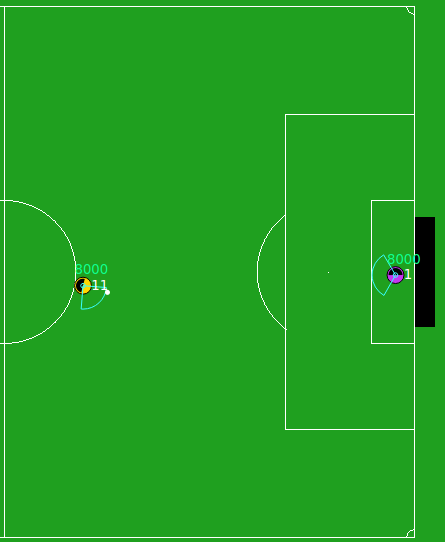
\includegraphics[width = 0.5\textwidth,height = 0.4\textheight, center]{../pictures/half-field.png}
            \caption{Screenshot von dem Spielfeld für den Subtask HFO \label{fig:somelabel}}
        \end{figure}
        \noindent
        Im Folgenden wir die Domäne samt Zustandsraum und Aktionen erklärt, sowie ihren Einschränkungen für die Anwendung von Machine Learning Algorithmen.\\
        % \cite{ http://www.cs.utexas.edu/users/ai-lab/?hausknecht:aamasws16 }
\newpage
        \subsection{Zustandsraum}
            % ``Unterschiedliche Zustandsräume, kommt drauf an wie viele Spieler aufm Feld sind (zitat vom HFO Paper)''\\
            % ``Angepasst für Maschinen (zitat HFO)'' \\
            % ``Umrechnung für Menschen'' \\
            % ``Fullstate flag''
            Der Zustandsraum der HFO Domäne kann in den \textbf{High Level State} und den \textbf{Low Level State} aufgeteilt werden. Der Unterschied ist lediglich in der Dimensionalität, da man aus dem Low Level State den High Level State ableiten kann. Die Zustandsräume werden durch folgende Formeln aufgespannt:\\
            \\
            \textit{Sei T die Anzahl der Teammitglieder, O die Anzahl der Gegner:}
            \begin{center}
                \textit{High Level State} $ := 10 + 6T + 3O \hspace{10mm} $ \\
                \textit{Low Level State}  $ := 58 + 8T + 8O \hspace{9mm} $ \\
            \end{center}
%            \textit{(Frage: Alles vom Paper abschreiben oder referenzieren?)} \\
 %           \\
            In unserem 1v1 High Level Setting haben wir damit 13 Zustandsparameter. Vier von diesen Parametern gehören zu dem Torwart, aber da seine Position implizit durch andere Ausprägungen gegeben ist, werden sie nicht beachtet. Redundante Information würde den Suchraum unnötig aufblähen und die Suche verlängern. Folgende 9 Zustände wurden bereitgestellt:

            \begin{table}[H]
                \begin{center}
                \hspace*{-1.5cm}
                \begin{tabular}{ |l|c|c|c| } 
                    \hline
                    \hfill Zustandsbeschreibung & Wertebereich & Kontinuierlich & Boole'sch \\ \hline
                    x Koordinaten & $[ -1, +1 ]$ & X & \hfill \\ \hline
                    y Koordinaten & $[ -1, +1 ]$ & X & \hfill \\ \hline
                    Sichtrichtung & $[ -1, +1]$ & X & \hfill \\ \hline
                    Nähe zum Ball & $[ -1, +1 ]$ & X & \hfill \\ \hline
                    Winkel zum Ball & $[ -1, +1 ]$ & X & \hfill \\ \hline
                    Kann eine Ballaktion ausgeführt werden & $[ -1, +1 ]$ & \hfill & X \\ \hline
                    Winkel zum Mittelpunkt des Tors & $[ -1, +1 ]$ & X & \hfill \\ \hline
                    Größte offene Winkel zwischen Torwart und Torpfosten & $[ -1, +1 ]$ & X & \hfill \\ \hline
                \end{tabular}
                \end{center}
                \caption{Zustandsraum von HFO 1vs1 \label{fig:somelabel}}
            \end{table}

            \hspace*{-1.5cm}
            \textit{(Muss hier eine Erklärung wie der Zustand kodiert war hin, also Normalisierung der Winkel?\\
            \hspace*{-1.5cm} Wäre dann eigentlich abschreiben ab 15.1.1 von https://github.com/LARG/HFO/blob/master/doc/manual.pdf)}
            % (src: https://github.com/LARG/HFO/blob/master/doc/manual.pdf ab 15.1.1)
        \subsection{Aktionsraum}
            % ``Gibt 6 nicht parametrisierte Aktionen, die wir benutzt haben''\\
            % ``Gibt noch andere parametrisierte''
            Es gibt 8 parametrisierte und 6 nicht parametrisierte Aktionen. Wir haben die Algorithmen über 5 der 6 Aktionen ohne zusätzlichen Argumente trainiert. Die Aktion \textit{CATCH} ist für Angreifer illegal und wurde deshalb weggelassen. Die folgende Aufzählung beschreibt alle Aktionen:
            \textit{(Genauere Erklärung von benutzen Aktionen kommt noch)}

            \begin{multicols}{2}
                \textbf{Parametrisierte}
                \begin{itemize}
                    \item Dash(power, degrees)
                    \item Turn(degrees)
                    \item Tackle(degrees)
                    \item Kick(power, degrees)
                    \item Kick\_To(x-coords, y-coords, speed)
                    \item Move\_To(x-coords, y-coords)
                    \item Dribble\_To(x-coords, y-coords)
                \end{itemize}
                \textbf{Nicht parametrisierte}
                \begin{itemize}
                    \item Move
                    \item Shoot
                    \item Dribble
                    \item Intercept
                    \item Catch
                    \item No-Op
                \end{itemize}
            \end{multicols}
            \noindent
            Jedes Spiel hatte eine maximale Zeit die in Frames aufgeteilt war und jeder Agent wird zu jedem Frame gefragt ob er eine neue Aktion ausführen will. Wenn ein Timeout von einem festen Zeitabstand kommt, wird pauschal die No-Op Aktion ausgeführt.

        \subsection{Einschränkungen}
            % ``Sparse Fitness''                 \\
            % ``Simulation Learning''            \\
            % ``Hochdimensional Kontinuierlich'' \\
            % ``Auch genannt Black Box RL''
            Diese Domäne hat viele Einschränkungen wenn man sie mit herkömmlichen Machine Learning Tasks vergleicht \textit{(Vergleich Moonrover, Roboterarm etc.)}. Zum einen erlaubt sie uns wegen der Implementierung nicht in die Zukunft zu propagieren und zu schauen wie gut eine Entscheidung ist. Wir haben eine Simulation die erst nachdem ein Spiel fertig ist ein Fitnesssignal sendet und wir daraufhin abzuleiten müssen ob die lange Aktionsketten die wir ausgeführt haben uns zum Erfolg führten. Diese Eigenschaft nennt sich \textbf{sparse Fitness} und findet sich in Beispielen wie \textit{(Zitat)}

            \begin{center} \textit{(Simulation based learning)} \end{center}
            \begin{center} \textit{(Kontinuierlicher Zustandsraum, hohe Abstraktion)} \end{center}
            % (cite https://gym.openai.com/docs/rl#black-box-optimization-and-the-cross-entropy-method)

    \section{Implementierung der Algorithmen}
        % ``Server in Haskell, HFOServer in C++, Agenten in Python''
        Der ausführliche Aufbau der Algorithmen wird näher im Appendix erklärt, hier schauen wir uns die Parametrisierung grobe Funktionsweise an. Die Simulation kann in die folgenden drei Teile unterteilt werden.

        \subsubsection*{Simulationsserver}
        Der Simulationsserver ist in C++ geschrieben und wurde 1-zu-1 aus [cite HFO] übernommen. Er wird durch Flags beim Starten parametrisiert.
        % (src: https://github.com/LARG/HFO)

        \subsubsection*{Agenten}
        Die Agenten sind in Python geschrieben und stellen eine Erweiterung von einem der Beispielskripte dar [cite HFO]. Diese Prozesse werden auch mit eigenen Kommandozeilenparametern aufgerufen.

        \subsubsection*{Koordinator}
        Der Koordinator ist für die Umsetzung des GAs und den jeweiligen Kodierungen zuständig, startet den Server und die Agenten Skripte und überwacht die Simulation. Er ist, wie alle folgenden Codebeispiele, in Haskell geschrieben.

        \subsubsection*{Simulation}
        Jedes Team hat pro Generation 25 Spiele gespielt und die gesamte Simulation bestand aus insgesamt 375000 Spielen.
        Die Episodenzeit wurde auf 500 Echtzeitsekunden beschränkt, da ansonsten die simulierte Zeit pro Spiel nicht praktikabel war. \\

        \noindent
        Für alle Simulationen galten die folgenden Rahmenbedingungen:

        \begin{center}
            \begin{tabular}{ |c|c| } 
                \hline
                Generationen       & $300$  \\ \hline
                Populationsgröße   & $50$   \\ \hline
                Teamepisoden       & $25$   \\ \hline
                Episodenzeit       & $500s$ \\ \hline
                Ball nicht berührt & $50s$  \\ \hline
                $\alpha$           & 0.25   \\ \hline
                $\beta$            & 0.10   \\ \hline
            \end{tabular}
        \end{center}

        \subsection{Wahrscheinlichkeitsverteilung von Aktionen}

            Der erste Algorithmus hat als Kodierung der Individuen eine diskrete Wahrscheinlichkeitsverteilung über 5 Aktionen benutzt. Wenn der Agent gestartet wurde samplet er jeden Zeitschritt ohne Wissen über jeglichen Zustand aus dieser Verteilung raus.

            \subsubsection*{Kodierung}

            \begin{align*}
                \text{Set von allen Aktionen }&X := \{\text{Move, Shoot, Dribble, Intercept, No-Op}\} \\
                &\forall x \in X: P(x) \geq 0 \\
                &\sum_{x \in X}^{} P(x) = 1
            \end{align*}

            \subsubsection*{Kreuzung}
            Die Kreuzung wurde auf zwei verschieden Arten umgesetzt, wobei sie im Vergleich an der vollständige Simulation weder neueartige Lösungen entwickelt haben, noch die Konvergenzzeit beeinflusst wurde.

            \subsubsection*{Generator}
            Die erste Methode kam aus der Idee wie man mit einer absehbaren Laufzeit eine Wahrscheinlichkeitsverteilung über $n$ Aktionen erstellt. Dafür werden $n-1$ zufällige Zahlen erstellt, als Liste verpackt, sortiert und jeweils eine $0$ von vorne und eine $100$ am Ende angehängt.

            \begin{minted}[escapeinside=||, xleftmargin=-50pt]{haskell}
                    > let n = 5
                    > take (n-1) <$> getRandomRs (0,100)
                    [87, 15, 55, 38]
                    > sort it
                    [15, 38, 55, 87]
                    > 0 : it ++ [100]
                    [0, 15, 38, 55, 87, 100]
            \end{minted}

            \noindent
            Anschließend wird diese Liste dupliziert und um ein Element nach rechts verschoben und paarweise voneinander abgezogen.
            \begin{minted}[escapeinside=||, xleftmargin=-50pt]{haskell}
                    > let l1 = [0, 15, 38, 55, 87, 100]
                    > drop 1 l1
                    [15,38,55,87,100]
                    > let l2 = it
                    > {-
                      [15, 38, 55, 87, 100]
                    - [ 0, 15, 38, 55,  87, 100]
                    = [15, 23, 17, 32,  13]
                    -}
                    > zipWith (-) l2 l1
                    [15, 23, 17, 32, 13]
                    > sum it
                    100
            \end{minted}

            \noindent
            Damit haben wir eine Wahrscheinlichkeitsverteilung über 5 Aktionen und können uns sicher sein dass sie aufsummiert immer $100$ ergibt. Die Kreuzung von zwei solcher Individuen wurde mit den jeweiligen Listen umgesetzt, aus denen sie generiert wurden. Dafür wurde elementweise der Durchschnitt berechnet und daraus entsteht dann eine neue Generatorliste aus der sich die Verteilung berechnen lässt.

            \begin{minted}[escapeinside=||, xleftmargin=-50pt]{haskell}
                    > let individualA = [0, 15, 38, 55, 87, 100]
                    > let individualB = [0, 7, 22, 35, 51, 100]
                    > zipWith (\x y -> (x + y) `div` 2) individualA individualB
                    [0, 11, 30, 45, 69, 100]
            \end{minted}

            \subsubsection*{Normalisierung}
            Die zweite Methode hat beide Verteilungen genommen, die Wahrscheinlichkeiten für jeweiligen Aktionen addiert und folgendermaßen normalisiert.\\
            \\
            \noindent
            Seien $\mathcal{A, B}$ die diskreten Wahrscheinlichkeitsverteilungen die verknüpft werden sollen: \\
            \begin{math}
            \\
            \hspace*{+4cm} \mathcal{C} := \{ \frac{(a_i + b_i)}{l} \; | \; a_i \in \mathcal{A}, b_i \in \mathcal{B}\} \hspace*{10mm} l := |\mathcal{A}|
            \\
            \end{math}
            \\
            \noindent

            \subsubsection*{Mutation}
            Die Mutation wurde auch mit jeweils dem Generator sowie Normalisierung umgesetzt. Im Kern ist jedoch die Funktion die das $\delta$ benutzt und es mit zufälligen Vorteichen in die Anzahl der Aktionen aufgeteilt. Man kann sich das $\delta$ als Veränderungsfaktor vorstellen, je höher er ist, umso unterschiedlicher wird die Wahrscheinlichkeitsverteilung.
            \begin{multicols}{2}
                \begin{minted}[escapeinside=||, xleftmargin=-50pt]{haskell}
                    > let delta = 20
                    > splitDelta delta 5
                    [-4, +4, +4, -4, -4]
                \end{minted}
                \begin{minted}[escapeinside=||, xleftmargin=-80pt]{haskell}
                    > let delta = 100
                    > splitDelta delta 4
                    [-25, +25, +25, -25]
                \end{minted}
            \end{multicols}

            \subsubsection*{Generator}

            Wir erstellen teilen das $\delta$ in $n-1$ Teile auf, fügen eine $0$ von vorne und $100$ von hinten hinzu und verknüpfen es analog wie in der Kreuzung mit dem Ausgangsgenerator. Diesmal müssen wir jedoch die Zahlen per Hand auf den Bereich von $0 - 100$ begrenzen.

            \begin{minted}[escapeinside=||, xleftmargin=-80pt]{haskell}
                > let delta = 100
                > splitDelta delta 4
                [-25, +25, +25, -25]
                > let mutGen = 0 : it ++ [100]
                > let child = [0, 14, 31, 49, 75, 100]
                > {-
                  [0, -25, +25, +25, -25, 100]
                + [0,  14,  31,  49,  75, 100]
                = [0, -11,  56,  74,  50, 200]
                min 0
                  [0,   0,  56,  74,  50, 200]
                max 100
                  [0,   0,  56,  74,  50, 100]
                sort
                  [0,   0,  50,  56,  74, 100]
                -}
                > sort $ zipWith (((max 0 . min 100) .) . (+)) child mutGen
                [0,0,50,56,74,100]
            \end{minted}

            Aus diesem Generator kann wieder eine Wahrscheinlichkeitsverteilung erstellt werden.

            \subsubsection*{Normalisierung}

            Bei der Lösung mit der Normalisierung generieren wir uns wieder die Liste aus dem $\delta$, summieren sie elementweise mit der Verteilung, überprüfen ob die Grenzen von $[0,100]$ überschritten wurden und normalisieren sie wie in der Kreuzung.

            \begin{minted}[escapeinside=||, xleftmargin=-80pt]{haskell}
                > let delta = 50
                > splitDelta delta 5
                [-10, +10, +10, -10, -10]
                > let mutGen = it
                > let child = [15, 8, 34, 21, 22]
                > zipWith (((max 0 . min 100) .) . (+)) child mutGen
                [5,18,44,11,12]
                > normalizeDist it
                [5,20,48,12,15]
            \end{minted}

            Damit bekommen wir wieder eine veränderte diskrete Verteilung zurück.
        \subsection{Cross Entropy mit DCT}
            ``Parametrisierung''
        \subsection{Neuroevolution mit DCT}
            ``Parametrisierung''
        \subsection{CoSyNE mit DCT}
            ``Parametrisierung''

    \section{Resultate}
        Im folgenden Teil beschreiben wir die Resultate und versuchen diese zu begründen. Durchschnittlich hat eine Trainigsphase mit 300 Generationen, Population der Größe 50 und 25 Episoden pro Team 30 Stunden gedauert. Die Simulationen wurden auf einem Laptop mit einem Intel i5 mit 2.9GHz und 4GB Arbeitsspeicher ausgeführt.\\[2mm]
        \noindent
        Nachdem wir pro Algorithmus die besten 5 Individuen ermitteln, lassen wir sie jeweils 10000 Spiele spielen, um die erfasste Fitness auf ihre Stabilität zu testen. \\[2mm]
        \noindent
        Sei $F_{Entwicklung}$ die entwickelte Fitness und $F_{Test}$ die neu getestete Fitness. Die Stabilität wird danach gemessen wie gering die Abweichung von $F_{Test}$ zu $F_{Entwicklung}$ ist. Je kleiner die Abweichung, umso stabiler und sicherer spielt das Individuum.\\

        \begin{center}
            \begin{math}
                \text{Abweichung} = \frac{F_{Entwicklung} - F_{Test}}{F_{Entwicklung}}
            \end{math}
        \end{center}

        \subsection{1v1}
            Unser Lernziel für die HFO Domäne war einen offensiven Spieler zu trainieren der gegen einen vom Server gesteuerten Torwart so gut es geht Tore schießt. Das haben wir mit vier in Kapitel 2 angesprochenend Algorithmen getestet und stellen die Resultate vor. 

\newpage
            \subsubsection*{Wahrscheinlichkeitsverteilung}
                \begin{multicols}{2}
                    \noindent
                    Die Wahrscheinlichkeitsverteilung war der erste naive Ansatz um zu überprüfen ob die Domäne bereits durch eine einfache Kodierung lösbar ist. Leider ging die Varianz in der Population nach der $10$ Generation gegen $0$ und die Verteilung sah folgendermaßen aus:
                    \begin{table}[H]
                        \begin{center}
                        \begin{tabular}{ |l|r| } 
                            \hline
                            \hfill Aktionen & P(Aktion)  \\ \hline
                            Move      & 22\% \\ \hline
                            Dribble   & 22\% \\ \hline
                            Intercept & 22\% \\ \hline
                            No-Op     & 22\% \\ \hline
                            Shoot     &  2\% \\ \hline
                        \end{tabular}
                        \end{center}
                    \end{table}

                    \begin{figure}[H]
                        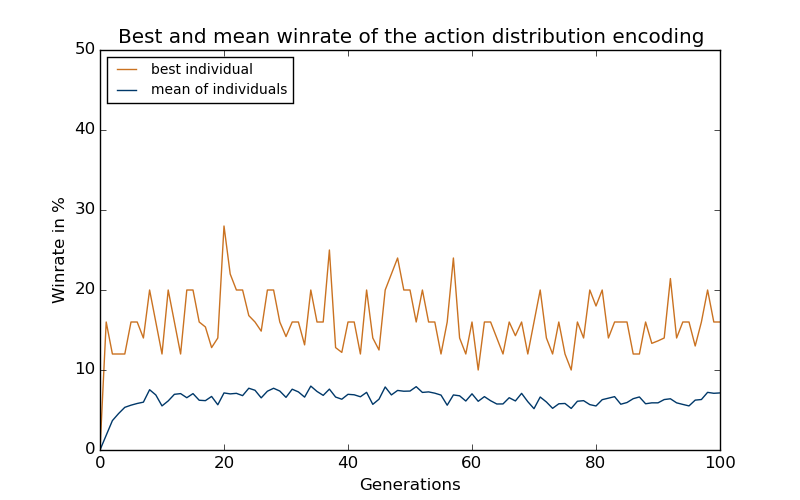
\includegraphics[scale=0.5]{../pictures/summary/actiondist-fitness.png}\\
                        \caption{Fitness Graph für die \\Wahrscheinlichkeitsverteilung}\label{fig:graph-ac}
                    \end{figure}
                \end{multicols}
                \noindent
                Die gesamte Population ist zu dem Ergebnis konvergiert, dass jede Aktion gleich wahrscheinlich ist, bis auf \textit{Shoot}. Die Schussaktion hat wahrscheinlich zu oft zu einem Schuss ins Aus geführt, was sofort das Spiel als zu Gunsten des Torwarts beendet.\\

                \noindent
                Die maximale erreichte Fitness beträgt 28\% und schwankt im Bereich von $[10,25]$. Leider stellt sich heraus dass die besten fünf Werte Ausreißer waren und keinesfalls die durchschnittliche Gewinnwahrscheinlichkeit darstellen. 

                \begin{table}[H]
                    \begin{center}
                    \begin{tabular}{ |l|r|r|r| } 
                        \hline
                        \hfill & Trained Fitness   & Tested Fitness  &          Error    \\ \hline
                          Nr.1 &          28.00\%  &          6.82\% &          75.64\%  \\  
                          Nr.2 &          25.00\%  &          5.54\% &          77.84\%  \\  
                          Nr.3 &          24.00\%  &          5.40\% &          77.50\%  \\ 
                          Nr.4 &          24.00\%  &          6.33\% &          73.62\%  \\ 
                          Nr.5 &          22.00\%  &          6.65\% &          69.78\%  \\ \hline
                          Mean &  \textbf{24.60\%} & \textbf{6.15\%} & \textbf{74.88\%}  \\ \hline
                    \end{tabular}
                    \end{center}
                    \caption{Stabilität der besten 5 Wahrscheinlichkeitsverteilungs Individuen \label{fig:actiondisttable}}
                \end{table}
                \noindent
                Die durchschnittliche Gewinnwahrscheinlichkeit liegt bei 6.15\% und wenn man den Spieler beobachtet kann man sich beim besten Willen nicht erklären, wie er überhaupt schafft Tore zu schießen, da er meistens versucht ins Tor zu laufen während ihm der Ball abgenommen wird. Es ist aber auch nicht verwunderlich, da der Spieler weder weiß wo der Torwart ist, ob er den Ball hat, noch wo er sich auf dem Spielfeld befindet. \\

                \begin{center} \textit{(Link zum Video)} \end{center}

\newpage
            \subsubsection*{Cross Entropy}
%                ``Graph zeigen, Interpretation bzw. Erklärung''
%                ``Aggressivität''
%                ``Nach ~ 50 Episoden stagniert''
                \begin{multicols}{2}
                    \noindent
                    \\[5mm]
                    Die Cross Entropy Methode hat sehr interessante Ergebnisse produziert, da sie durchschnittlich eine 4\% bessere Fitness hat, die Stabilität jedoch um 3\% schlechter ist, als wie die Wahrscheinlichkeitsverteilung.\\[2mm]
                    Sie ist nach ungefähr 50 Generationen konvergiert und die maximale erreichte Fitness beträgt 32\% und schwankt im Bereich von $[15,30]$. 
                    \begin{figure}[H]
                       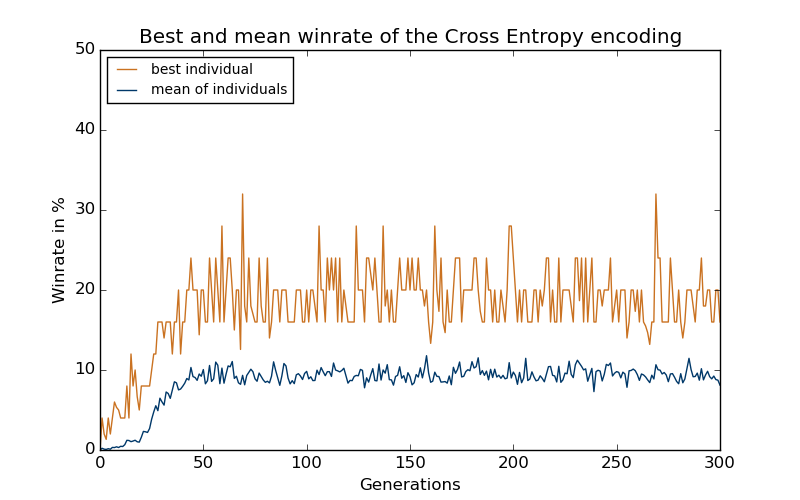
\includegraphics[scale=0.5]{../pictures/summary/cross-entropy-fitness.png}
                       \caption{Fitness Graph für Cross Entropy}\label{fig:graph-ce}
                    \end{figure}
                \end{multicols}

                \begin{table}[H]
                    \begin{center}
                    \begin{tabular}{ |l|r|r|r| } 
                        \hline
                        \hfill & Trained Fitness   & Tested Fitness  &          Error    \\ \hline
                          Nr.1 &          32.00\%  &          7.26\% &          77.31\%  \\  
                          Nr.2 &          32.00\%  &          7.46\% &          76.69\%  \\  
                          Nr.3 &          28.00\%  &          7.37\% &          73.68\%  \\ 
                          Nr.4 &          28.00\%  &          7.27\% &          74.04\%  \\ 
                          Nr.5 &          28.00\%  &          3.46\% &          87.64\%  \\ \hline
                          Mean &  \textbf{29.60\%} & \textbf{6.56\%} & \textbf{77.87\%}  \\ \hline
                    \end{tabular}
                    \end{center}
                    \caption{Stabilität der besten 5 Cross Entropy Individuen \label{fig:crossentropytable}}
                \end{table}
                \noindent
                Von den Werten sieht man kaum einen Unterschied zu der Wahrscheinlichkeitsverteilung, aber in der Simulation merkt man ein extrem aggressives Verhalten vom Spieler. Der Agent schießt den Ball sehr oft und versucht bereits nachdem er die Mitte des Spielfeldes überquert hat ein Tor zu schießen, unabhängig davon ob er in einer guten Position ist. Das führt natürlich wieder dazu dass er öfter ins Aus schießt, ist aber wesentlich interessanter anzuschauen, da er von Spiel zu Spiel unberechenbar ist. \\

                \begin{center} \textit{(Link zum Video}) \end{center}
\newpage
            \subsubsection*{Neuroevolution}
                \begin{multicols}{2}
                    \noindent
                    \\[5mm]
                    Der Ansatz die Gewichte naiv als DCT Koeffizienten darzustellen führe zu den besten Ergebnissen. Das stärkste Individuum hat knapp jedes zweite Spiel gewonnen und ist mehr als 3-mal stabiler als die Cross-Entropy Lösung. Die Fitness hat sich nach ungefähr 150 Generationen im Bereich von $[30,45]$ eingependelt.
                    \begin{figure}[H]
                       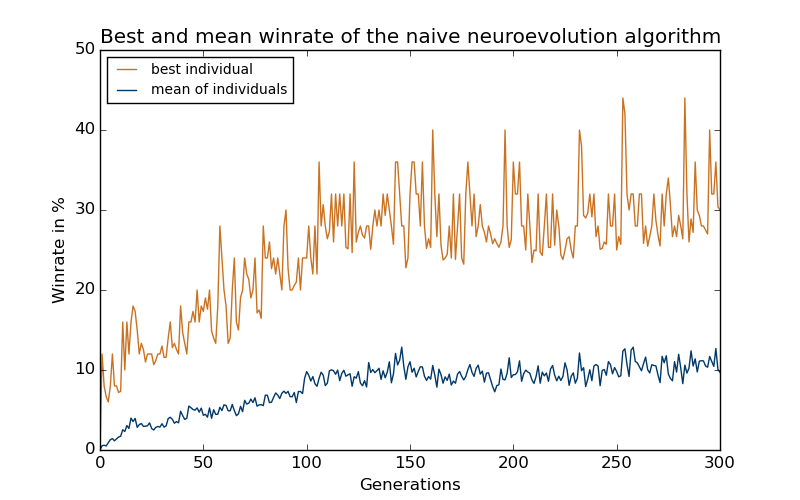
\includegraphics[scale=0.5]{../pictures/summary/neural-fitness.png}
                       \caption{Fitness Graph für Cross Entropy}\label{fig:graph-ne}
                    \end{figure}
                \end{multicols}

                \begin{table}[H]
                    \begin{center}
                    \begin{tabular}{ |l|r|r|r| } 
                        \hline
                        \hfill & Trained Fitness   & Tested Fitness  &          Error    \\ \hline
                          Nr.1 &          44.00\%  &         19.04\% &          56.72\%  \\  
                          Nr.2 &          44.00\%  &         20.18\% &          54.14\%  \\  
                          Nr.3 &          42.00\%  &         20.07\% &          52.21\%  \\ 
                          Nr.4 &          40.00\%  &         20.10\% &          49.75\%  \\ 
                          Nr.5 &          40.00\%  &         21.28\% &          46.80\%  \\ \hline
                          Mean &  \textbf{42.00\%} & \textbf{20.13\%} & \textbf{51.93\%}  \\ \hline
                    \end{tabular}
                    \end{center}
                    \caption{Stabilität der besten 5 Neurevolution Individuen \label{fig:neuroevotable}}
                \end{table}

                \noindent
                Die stabile Fitness ist bei knapp 20\% und damit gewinnen diese Individuen durchschnittliche jedes fünfte Spiel. Die Spielweise von diesem Ansatz könnte man \textit{geplant} erklären, da der Spieler oft zum Tor rennt, kurz vor dem Strafraum stehen bleibt und von Ecke zu Ecke pendelt bis er den Torwart etwas aus dem Tor gelockt hat um ein Tor zu schießen. Wenn er mal verliert, ist es weil er sofort zum Beginn des Spieles sich ins Aus schießt, oder zu nah am Tor ist, sodass ihm der Ball abgenommen wird.\\

                \begin{center} \textit{(Link zum Video)} \end{center}
\newpage
            \subsubsection*{CoSyNE}
%                ``Graph zeigen, Interpretation bzw. Erklärung''
                \begin{multicols}{2}
                    \noindent
                    \\[5mm]
                    Der CoSyNE Algorithmus ist in der durchschnittlichen Fitness knapp 5\% hinter der Neuroevolution, hat dafür aber ganze 15\% in der Stabilität verloren. Aus der Natur von dem CoSyNE gab es selbst bei der 300 Generation noch exterm unterschiedliche Individuen und eine Konvergenz war nicht zu erkennen. 
                    \begin{figure}[H]
                       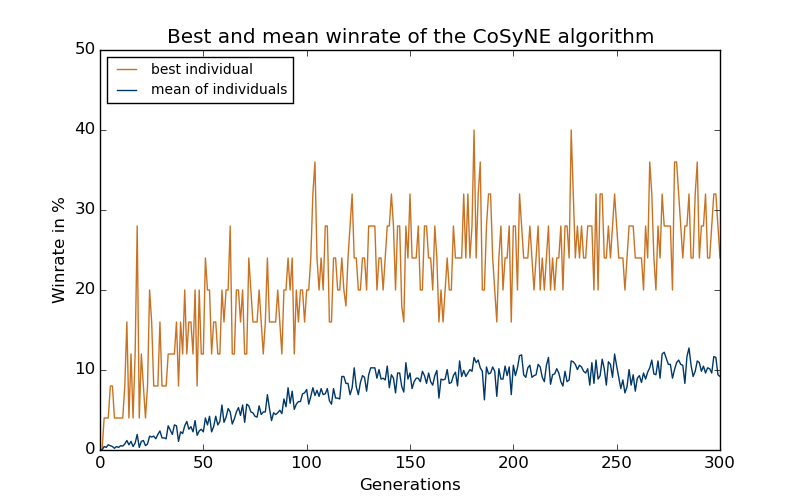
\includegraphics[scale=0.5]{../pictures/summary/cosyne-fitness.png}
                       \caption{Fitness Graph für Cross Entropy}\label{fig:graph-co}
                    \end{figure}
                \end{multicols}

                \begin{table}[H]
                    \begin{center}
                    \begin{tabular}{ |l|r|r|r| } 
                        \hline
                        \hfill & Trained Fitness   & Tested Fitness  &          Error    \\ \hline
                          Nr.1 &          40.00\%  &         14.21\% &          64.47\%  \\  
                          Nr.2 &          40.00\%  &         14.22\% &          64.45\%  \\  
                          Nr.3 &          36.00\%  &         12.68\% &          64.48\%  \\ 
                          Nr.4 &          36.00\%  &         15.42\% &          57.16\%  \\ 
                          Nr.5 &          36.00\%  &          5.75\% &          84.02\%  \\ \hline
                          Mean &  \textbf{37.60\%} & \textbf{12.45\%} & \textbf{66.98\%}  \\ \hline
                    \end{tabular}
                    \end{center}
                    \caption{Stabilität der besten 5 Neurevolution Individuen \label{fig:neuroevotable}}
                \end{table}
                \noindent
                Die beste Individuen haben lediglichlich nur knapp 12\% ihrer Spiele gewonnen und man kann eine ähnliche Taktik wie die Neuroevolution Agenten erahnen, nur wesentlich schlechter umgesetzt. Es passiert häufig, dass der Agent kurz vor dem Strafraum stehen bleibt und sich für eine sehr lange Zeit nicht bewegt. Da der Torwart nicht zu weit von dem Tor rausgeht, befinden sie sich im Deadlock bis der Agent versucht ein Tor zu schießen. Das Schießen am Anfang des Spiels tritt hier auf gehäuft auf.

                \begin{center} \textit{(Link zum Video)} \end{center}
\newpage
        \subsection{Vergleich}
%            ``Sicherheit <-> Aggressivität steht im Kontra zur Stabilität der Algorithmen''\\
%            ``Wenn Zeit ein Faktor wäre'' \\
%            ``Wenn Sicherheit ein Faktor wäre'' \\

             Im Vergleich zwischen allen Algorithmen sieht das Ranking folgendermaßen aus:

                \begin{table}[H]
                    \begin{center}
                    \begin{tabular}{ |l|r|r|r| } 
                        \hline
                        \textbf{Algorithmus}          & E(Trained Fitness) & E(Tested Fitness) & E(Error)    \\ \hline
                        Neuroevolution                &          42.00\%   &         20.13\%   &    51.93\%  \\ \hline
                        CoSyNE                        &          37.60\%   &         12.45\%   &    66.98\%  \\ \hline
                        Cross-Entropy                 &          29.60\%   &          6.56\%   &    77.87\%  \\ \hline
                        Wahrscheinlichkeitsverteilung &          24.60\%   &          6.15\%   &    74.88\%  \\ \hline
                    \end{tabular}
                    \end{center}
                    \caption{Alle Algorithmen gegenübergestellt \label{fig:vergleichstabelle}}
                \end{table}

            \noindent
            Neuroevolution gewinnt eindeutig in allen getesteten Merkmalen und hat während den Aufnahmen den raffiniertesten Eindruck gemacht. Wir sehen pauschale Aggressivität wie bei Cross-Entropy zwar interessante Züge macht, jedoch nicht tauglich ist für den Einsatz auf dem echten Spielfeld. \\[2mm]

            \noindent
            Sicherheit und die \textit{Planung} machen auf lange Sicht viel mehr Sinn und sollten verstärkt werden. Der CoSyNE Algorithmus unterstützt diese Art von Entwicklung in dieser Dimensionalität schlechter als die naive Suche über alle Parameter. Es ist zu überprüfen ob diese Aussage für gleichzeitiges Lernen in einem 2v1 Setting übereinstimmt.\\[2mm]

            \begin{center} \textit{(Link zur Best-Of-Compilation Video)} \end{center}






    \addtocontents{toc}{\protect\newpage}
\chapter{Diskussion}
    In diesem Kapitel schauen wir uns die Ergebnisse aus dem Vergleich zwischen den verschiedenen Algorithmen und deren Einschränkungen an, erwägen den potenziellen Nutzen für ähnliche Probleme und stellen Verbesserungsvorschläge dar. Das Schlusswort umfasst verwandte Felder die im Bezug zu unseren Algorithmen stehen.
    \section{Anwendungsmöglichkeiten}
        Unsere Aufgabe hat Einschränkungen, die für viele Probleme aus der realen Welt zutreffen, wie seltene Fitnesssignale, kontinuierliche und verrauschte Zustandsräume, sowie aufeinander aufbauende Aktionsketten. Daher glauben wir dass die Anwendungsgebiete, wie autonomes Verhalten voneinander abhängigen Robotern, selbstfahrende Autos oder das Entdecken von neuen Lösungswegen mithilfe von simplen Fitnessfunktionen, mit diesen Techniken weitergebracht werden kann. \\

        \noindent
        Vorallem war es interessant zu sehen, dass KNNs entwickelt werden können, die lediglich aus 20 Koeffizienten bestehen, extrem korellierte Gewichte produzieren und trotzdem lernen können. Ohne die Tests könnten man aus Abbildung \ref{fig:dct-my-case} ableiten, dass es extrem unwahrscheinlich ist, dass das befüllte Netz in irgendeiner Art Nutzen bringt. Deshalb können wir die Annahme, dass Gewichte in neuronalen Netzen keine große Abweichung zueinander haben müssen, bestätigen \cite{cosyne1}. Es wäre interessant zu schauen, ob bei Netzen die viel größer sind, ähnliche Ergebnisse möglich wären. \\

        \noindent
        CoSyNE wirft mit der treppenförmigen Fitnesskurve die Idee auf, ob eine stetige Verbesserung, oder explizit keine Verschlechterung als Garantie gegeben werden kann. Diese Eigenschaft wurde bisher nicht in der Literatur erwähnt und wäre unter dem statistischen Sicherheitsaspekt interessant zu untersuchen.

\newpage

    \section{Ausblick} \label{ausblick}
        Diese Arbeit hat leider einen festen Zeitrahmen gehabt und wir konnten vieles nicht ausprobieren. Wir sprechen mögliche Verbesserungen an, die man in zukünftigen Arbeiten beachtet werden können.

        \subsection*{Genetische Algorithmen}
            Die genetische Suche wurde mit ausgewogenen Parametern durchgeführt, die jedoch keine besondere Spezialisierung für die Anwendung bekommen haben. Darunter fällt der Mutationsparamter in CoSyNE, der in der Literatur sehr hoch gewählt war \cite{cosyne2} und die Begrenzung der Koeffizienten auf [-3,3] die wir gewählt haben, weil es keine Literatur dafür gab. 
        \subsection*{Aufbau des neuronalen Netzes}
            Der Aufbau des KNNs kann mit von der Schicht aus LSTM Neuronen in Tiefe und Größe verändert werden, da wir potenziell bessere Lernfähigkeiten bekommen können. Vorallem in der Kombination mit der DCT Kompression besteht die Möglichkeit Netze mit über 1 Million Gewichten erfolgreich zu kodieren \cite{cosyne4}. \\[2mm]
            \noindent
            Ausser DCT gibt es noch eine andere Suchraumverringerung die auf Wavelets basiert und vielversprechendere Ergebinsse in vielen Arcade Learning Environments geschafft hat \cite{wavelet}. Die Wavelets kodieren den Zustandsraum auch in hochfrequenten Domänen, behalten aber im Gegensatz zu Fouriertransformationen die Stetigkeit in der Ordnung der Daten, was zu schnelleren Lösungen in der Octopusarm Aufgabe geführt hat.

        \subsection*{Cross Entropy Method}
            Die Cross Entropy Method Lösung wurde lediglich in der einfachsten Form umgesetzt und es fand weder Repopulation mit neuen Individuen statt, noch haben wir einen Mutationsschritt gehabt. Das Hinzufügen von diesen Methoden würde wahrscheinlich zu besseren Lösungen führen. Viele Verberbesserungen finden sich auch in \cite{cem}.

        \subsection*{Aktionsraum}
            Der High-Level Aktionsraum wurde während der Arbeit im HFO Framework erweitert, sodass wir Aktionen wie \textit{Go\_To\_Ball} oder \textit{Reduce\_Angle\_To\_Ball} nicht benutzt haben. Da die Dokumentation der übrigen Aktionen sehr spärlich ausgefallen ist, würden eigene Aktionen eine bessere Möglichkeit bieten über die Effektivität der Algorithmen zu argumentieren. Sie würden auch sehr wahrscheinlich mehr Taktiken zulassen.

        \subsection*{Multi-Agenten Systeme}
            Da die Simulation skalierend modelliert wurde, erlaubt sie uns einfaches Testen mit mehreren Agenten, wie 2vs1, oder 4vs4. Leider hätten ausführliche Tests dieser Domänen den zeitlichen Rahmen der Bachelorarbeit maßlos gesprengt.

\newpage

    \section{Schlusswort}
        TODO


        \subsection*{Implementierung für OpenAI Gym}
            Während der Entwicklung dieser Arbeit gab es eine Implementierung der HFO Domäne für das 1vs1 Szenario in der OpenAI Gym, das ein bekanntes machine learning Framework in Python ist. Die Umsetzung von unseren Algorithmen dafür wäre der nächste logische Schritt um die neuroevolutionären Methoden mehr in den Fokus zu Rücken. Diese spezielle Implementierung erlaubt uns Schritte vorzusimulieren, da der Torwart deterministisch ist. Damit können andere Trainingstechniken, wie Backpropagation, benutzt werden, die einen interessanten Vergleich anstellen.

        \subsection*{ConvNet, CoSyNE, DCT und Wavelets}
            In \cite{cosyne4} wird CoSyNE und DCT für die Komprimierung von über 1 Million Gewichten in einem Convolutional Neural Network benutzt und hat beeindruckende Ergebnisse für die Steuerung von einem Auto mit Bilddaten erzielt. Deshalb würde es sich anbieten die Verknüpfung von CoSyNE und DCT auf anderen Aufgaben, die auf hochdimensinalen korrelierten Daten basieren, anzuwenden. \\

            \noindent
            Wavelets, die von Jürgen Schmidhuber als als logischer Nachfolger für die DCT Transformation im Gewichtssuchraum entwickelt wurden \cite{wavelet}, sollten auch einem Vergleich mit naiven GAs und CoSyNE unterzogen werden, da bei unseren Beispielen der naive GA bessere Individuen entwickelt hat.

        \subsection*{RoboCup}
            RoboCup hat sich als Ziel gesetzt echte Roboter gegen die Fußballweltmeister im Jahr 2050 antreten zu lassen und ich bin nach dieser Arbeit der Ansicht, dass es gar nicht so unwahrscheinlich ist. Wenn wir die aktuellen Robotikfortschritte anschauen, wie Atlas von Boston Dynamics \cite{robot}, der bereits externe Krafteinwirkungen abfangen kann, ist der Weg nicht mehr weit zu gemeinsamen sportlichen Aktivitäten.\\

            \noindent
            Man muss sich vor Augen führen, dass die Entwicklung von Machine Learning in den letzten 12 Jahren einen extremen Sprung gemacht hat, was Bilderkennung \cite{NIPS2012_4824}, eine Go KI, Stimmsynthese und allgemeine Spieler für das Atari Arcade Learning Environment \cite{Naddaf2010}, angeht. Wir sind heute noch ganze 34 Jahre von der Deadline entfernt und wenn wir mit ähnlicher Effektivität diese Zeit nutzen werden wie die letzten Jahre, bin ich überzeugt davon, dass Fußball eine eigene Roboter Liga bekommen wird.

%
% =================================================================================================
% place your appendix here
% -------------------------------------------------------------------------------------------------
%
    \appendix
    % -------------------------------------------------------------------------------------------------
%      MDSG Latex Framework
%      ============================================================================================
%      File:                  appendix.tex
%      Author(s):             Michael Duerr
%      Version:               1
%      Creation Date:         30. Mai 2010
%      Creation Date:         30. Mai 2010
%
%      Notes:                 - Place your appendix here
%                             - Use the same commands (`chapter', `section', ...) as in main text
% -------------------------------------------------------------------------------------------------
%
% \cite{andr04}
\chapter{Appendix}
``Da der Fokus sehr stark auf dem Machine Learning Bereich lag, aber die Domäne viele Tücken hatte und die Implementierung einen Großteil der Zeit in Anspruch genommen hat, wird es hier behandelt''

\section{Architektur}
    ``Die Architektur des gesamten Projektes wurde in Haskell geplant, da ich mit externen und unsicheren Implementierungen arbeite''\\
    ``Automatische Docs, weil ich gute Kommentare schreibe''
    ``Hat geholfen Fehler schneller zu finden und Codereuse ist super geil gewesen'' \\
    ``Bild von der Kommunikation zeichnen''
    \subsection{Haskell Server}
        ``Module'' \\
        ``Typklassen sind geil'' \\ 
        ``Globale Config ist nice'' \\
        ``Automatische Serialisierung mit Aeson''
    \subsection{Python Agent}
        ``Module''     \\
        ``CMD Parser'' \\
        ``Keras''
    \subsection{Kommunikation}
        ``Haskell <-> Python: JSON ist von Python nativ als Dict unterstützt''
        ``Python <-> Server: FFI Python to C++ (HFO) + (Zitat)''
    \subsection{Parallelisierungsmöglichkeiten}
        ``Bottleneck ist die Kommunikation über JSON-Files''

\section{Statistik}
    ``Für Cross Entropy hab ich Varianz und STD mit Seed gebraucht, für MonadRandom gabs keine Implementierung, dsw hab ich eine eigne gemacht''
    \subsection{Lineares Laufzeit und Speicherkomplexität für Evaluation}
        ``Folds sind supernice, minimale Erklärung, Links zu Gabriels Blog, Vorzeigen von Effizienz''
    \subsection{Stabile Varianzfunktion}
        ``Catastrophic Cancellation, erste Lösung, zweite Lösung von Gabriel mit E-Mail Austausch''

\section{Problematiken}
    ``Server ist scheiße, nicht besonders gut dokumentiert''
    \subsection{HFO Server}
        ``Erfolgreicher Durchlauf ist abhängig vom Computer, bzw. von der Leistung'' \\
        ``Undefinierte Lags zwischen Step 2k-8k'' \\
        ``Bedienung vom Visualizer ist nicht richtig erklärt'' \\
        ``Visualizer produziert nicht benutzbare logs, nur das erste Spiel ist `abspielbar', rest ist korrupt '' \\
        ``Einloggen von Spielern nimmt sehr viel Zeit in Kauf, dafür muss ein Austausch von Policies on-the-fly passieren'' \\
        ``Visualzer bricht bei 24k Steps ab, aber ohne ihn funktioniert die Simulation nicht, laggt nur rum'' \\
        ``Es gibt keine Zeitangaben wie lange ein Agent nicht aktiv sein darf, wenn er keine Entscheidung abgibt wird er ignoriert, dieser Fall sollte behandelt werden für kompetative Benutzung''
    \subsection{HFO Python Library}
        ``Kodierung von Zuständen in denen sich der Agent befindet gibt ein Hexdump zurück, man muss per Hand die ENUMS herausfinden und hardcoden'' \\

    % further appendix
%
% =================================================================================================
% comment \listoffigures and/or \listoftables if not wanted
% -------------------------------------------------------------------------------------------------
%
%    \backmatter
%    \listoffigures                                % list of figures (uncomment if wanted)
%    \listoftables                                 % list of tables (uncomment if wanted)
%    \lstlistoflistings                            % list of listings (uncomment if wanted)
%
% =================================================================================================
% place your bibliography here
% -------------------------------------------------------------------------------------------------
%
    \begin{spacing}{0.9}                          % save some space
       \bibliographystyle{ieeetr}                 % enumerated citings
%       \bibliographystyle{geralpha}               % for german thesis
       %\bibliographystyle{alpha}                 % for english thesis
       \bibliography{bibliography}                % the location of bib file
    \end{spacing}
\end{document}
%
% =================================================================================================
% end of document
% -------------------------------------------------------------------------------------------------
%
